\documentclass[12pt,reqno]{amsart}
\usepackage[margin=3cm]{geometry}

\usepackage{amsmath, amssymb, amsfonts, tikz,enumerate, graphicx, textcomp, caption, wrapfig, amsthm, todonotes, verbatim, cleveref, caption, float, mathabx}
\usetikzlibrary{calc, arrows}
\usepackage[procnames]{listings}
\usepackage{color, subfig}
\usepackage[section]{placeins}

\usepackage{color}
\definecolor{purple}{rgb}{0.5,0,1}

\newenvironment{dami}{
  \medskip
\begin{color}{blue}
    \textcolor{purple}{\textbf{Dami:}} 
}{
\end{color}
  \medskip
}


\newenvironment{cat}{
  \medskip
\begin{color}{red}
    \textcolor{red}{\textbf{Catherine:}} 
}{
\end{color}
  \medskip
}

\definecolor{keywords}{RGB}{255,0,90}
\definecolor{comments}{RGB}{0,0,113}
\definecolor{red}{RGB}{160,0,0}
\definecolor{green}{RGB}{0,150,0}
\lstdefinelanguage{Magma}%
  {%
   otherkeywords={:=,+:=,-:=,*:=},%
          % functions
   procnamekeys={function,func,intrinsic,procedure,proc},%
         % Booleans
   morekeywords={true,false},%
          % relations
   morekeywords=[2]{adj,and,cat,cmpeq,cmpne,diff,div,eq,ge,gt,in,is,join,le,lt,%
          meet,mod,ne,notadj,notin,notsubset,or,sdiff,subset,xor},%
          % keywords
   morekeywords=[3]{assigned,break,by,case,catch,continue,declare,default,%
          delete,do,elif,else,end,eval,exists,exit,for,forall,fprintf,if,local,%
          not,print,printf,quit,random,read,readi,repeat,restore,save,select,%
          then,time,to,try,until,vprint,vprintf,vtime,when,where,while},%
          % directives
   morekeywords=[4]{clear,forward,freeze,iload,import,load},%
          % error checks
   morekeywords=[5]{assert,assert2,assert3,error,require,requirege,requirerange},%
          % constructors
   morekeywords=[6]{car,comp,cop,elt,ext,frac,hom,ideal,iso,lideal,loc,map,%
          ncl,pmap,quo,rec,recformat,rep,rideal,sub},%
          % other constructors (semi-reserved)
   morekeywords=[7]{AbelianGroup,AdditiveCode,AffineAlgebra,Algebra,%
          AssociativeAlgebra,Character,CliffordAlgebra,Design,Digraph,%
          ExtensionField,FPAlgebra,FiniteAffinePlane,FiniteProjectivePlane,%
          Graph,Group,GroupAlgebra,IncidenceStructure,LieAlgebra,LinearCode,%
          LinearSpace,MatrixAlgebra,MatrixGroup,MatrixRing,Monoid,%
          MultiDigraph,MultiGraph,NearLinearSpace,Network,PartialMap,%
          PermutationGroup,PolycyclicGroup,QuaternionAlgebra,Semigroup,%
          ZModule},%
          % functions
   morekeywords={[8]function,func,intrinsic,procedure,proc,return},%
      sensitive,%
      morecomment=[l]//,%
      morecomment=[s]{/*}{*/},%
      morecomment=[s]{\{}{\}},%
      morestring=[b]"%
  }[keywords,procnames,comments,strings]%
\lstset{language=Python, 
        basicstyle=\ttfamily\small, 
        keywordstyle=\color{keywords},
        commentstyle=\color{comments},
        stringstyle=\color{red},
        breaklines=true,
        showstringspaces=false,
        identifierstyle=\color{green},
        procnamekeys={def,class}}
%\usepackage[T1]{fontenc}
%\usepackage[urw-garamond]{mathdesign}
\usepackage{tikz-cd}\tikzset{node distance=2cm, auto}
\DeclareMathOperator{\Aut}{Aut}
\DeclareMathOperator{\Hom}{Hom}
\DeclareMathOperator{\Jac}{Jac}
\DeclareMathOperator{\Alt}{Alt}
\DeclareMathOperator{\Corr}{Corr}
\DeclareMathOperator{\im}{im}
\DeclareMathOperator{\uncurry}{uncurry}
\DeclareMathOperator{\Pic}{Pic}
\DeclareMathOperator{\Div}{Div}
\newcommand{\C}{\mathbb{C}}
\newcommand{\Z}{\mathbb{Z}}
\newcommand{\F}{\mathbb{F}}
\newcommand{\G}{\mathbb{G}}
\newcommand{\Q}{\mathbb{Q}}
\newcommand{\R}{\mathbb{R}}
\newcommand{\n}{\newline}
\newcommand{\mc}{\mathcal}
\newcommand{\te}{\text}
\newcommand{\bb}{\mathbb}
\renewcommand{\P}{\mathbb{P}}
\newcommand{\BBF}{\overline{\F_p}}
\newcommand\mapsfrom{\mathrel{\reflectbox{\ensuremath{\mapsto}}}}
\definecolor{codegray}{gray}{0.9}
\newcommand{\code}[1]{\colorbox{codegray}{\texttt{#1}}}
\newtheorem{theorem}{Theorem}
\newtheorem*{thm*}{Theorem}
\newtheorem*{proposition}{Proposition}
\newtheorem{lemma}[theorem]{Lemma}
\newtheorem*{lemma*}{Lemma}
\newtheorem*{qlemma*}{``Lemma"}
\newtheorem{cor}[theorem]{Corollary}
\newtheorem{conjecture}[theorem]{Conjecture}
\newtheorem{postulate}[theorem]{Postulate}
\newtheorem*{question}{Question}
\theoremstyle{definition}
\newtheorem{defn}{Definition}
\newtheorem{example}[theorem]{Example}
\theoremstyle{remark}
\newtheorem*{remark}{Remark}
\newtheorem*{notation}{Notation}
\newtheorem*{note}{Note}
\newcommand{\sss}{\ss$\text{ }$}
\newcommand{\ti}{\todo[inline]}
\newcommand{\DD}{\Delta\kern -8.3pt {\diamond} \kern -4.5pt \cdot \:}
\newenvironment{myproof}[1][``\proofname '']{%
  \proof[ #1]%
}{\endproof}




\title{Automorphisms of the Jacobian} 
\author{Dami Lee and Catherine Ray}

\begin{document}

	
	\maketitle
	
\begin{abstract}
In this paper, we calculate and interpret the interaction between the automorphism group of a Riemann surface and the automorphism group of its Jacobian. We exposit and expand some calculational techniques from computational arithmetic geometry and hyperbolic geometry. We calculate the automorphism groups of some well-known surfaces such as Klein's quartic, Fermat's quartic, and Bring's curve. For further examples, we exploit the fact that the previously mentioned surfaces can be described as cyclically branched coverings over punctured spheres. We also discuss the modular curve $X_0(63),$ which is not a cyclic cover over a sphere. We find several principal polarizations on many Jacobians of these Riemann surfaces, and the automorphism groups with respect to each of these polarizations. We discuss and answer questions on Jacobians with multiple principal polarizations. 

\end{abstract} 
	
	
\tableofcontents

%\begin{acknowledgements} \end{acknowledgements}



\section*{Acknowledgements} 
The first author would like to thank Matthias Weber for his guidance at the beginning of this project. The second author would like to thank Magma and Sage contributors Edgar Costa, John Voight, Nicolas Mascot, and above all Jeroen Sijsling, who generously offered incredibly detailed and consistent help in computing the automorphism groups of Jacobians.

\section{Introduction} 

%A classical question in algebraic geometry is the Schottky problem that asks which principally polarized abelian varieties arise as Jacobian varieties of Riemann surfaces. Given Riemann surfaces of genus $g,$ let $\mathcal{M}_g$ be the moduli space of genus $g$ curves and let $\mathcal{A}_g$ be the moduli space of abelian varieties of dimension $g,$ which are principally polarized. Then there is a mapping $\mathcal{M}_g \rightarrow \mathcal{A}_g.$ Torelli's theorem tells us that this map is injective and the Schottky problem is to determine the image of the mapping. 

We are interested in the interaction between the automorphism groups of Riemann surfaces and the automorphism groups of their Jacobian varieties. Hurwitz's theorem gives us a bound of the order of the automorphism group of a compact Riemann surface of genus greater than one. However, computing the automorphism group of a Riemann surface is in general difficult. We exposit and improve two complementary methods to calculate the automorphism group of a given Riemann surface.

One method is from computational arithmetic geometry. This program is based on the work of Bruin-Sijsling-Zotine introduced in \cite{jeroen}. The program takes an explicit plane curve and provides the automorphism group of its Jacobian with respect to the curve's canonical principal polarization. Then we use Torelli's theorem tells us about an abstract isomorphism between these automorphism groups if the curve is hyperelliptic. If the curve is not hyperelliptic, then we get an extra $\Z/2$ factor. % discussed in section ~\ref{sec:torelli}.

The other method is from hyperbolic geometry. In \cite{dami}, the first author develops the tessellation-flag method to compute the automorphism group of Fermat's quartic. This method works particularly well on highly symmetric surfaces, e.g. those whose Weierstrass points have uniform weight. Lee presents Fermat's quartic as an eightfold cyclically branched cover over a thrice punctured sphere and finds a regular hyperbolic tessellation on the surface that is preserved under the automorphism group. Using this tessellation, Lee computes the automorphism group of Fermat's quartic in a generator-relation format. In this paper, we extend this to surfaces that have Weierstrass points of different weights. 

These two methods clarify each other. On one hand, Lee's method of investigating curves as cyclic covers over spheres eases the computation. We discuss such covers in section~\ref{sec:chap3} and further details can be found in \cite{dthesis}. These surfaces have many symmetries, hence one can identify the hyperbolic structure, flat structure, an explicit basis of holomorphic 1-forms, algebraic description, etc. The cyclicity on each surface makes it easy to compute period matrices which we use as inputs in our programs. On the other hand, the Jacobian program allows us to check the results obtained from Lee's method. 

To show the range of the Jacobian program, we also treat the case of the modular curve $X_0(63)$, which is not a cyclic cover over a sphere. Modular curves give information about modular forms and provide friendly examples of moduli spaces. The compactified modular curves are Riemann surfaces, and therefore, we may apply our methods to them. The case of all $X_0(N)$ except $N = 63$ was completed by \cite{km}. The case of $X_0(63)$ was done by Elkies soon after using two different proofs. We present a different proof going through the Jacobian.
% Understanding the abstract isomorphism (from Torelli's theorem) explicitly allows us to use Lee's method to visualize the tessellation induced on the Jacobian by its underlying curve. 

From the endomorphism ring of a Jacobian, we can directly understand the splitting of $\Jac(C)$ into simple abelian varieties (Corollary 4.8, \cite{jeroen}). In the case that these varieties are elliptic curves, which occurs surprisingly often, we can write down the point count of $\Jac(C)$ over any finite field, and therefore the L-function of $\Jac(C)$. The endomorphism ring is calculated along the way to the automorphism group.

%\ti{this sentence either needs to be expanded or removed: The exterior derivative of a holomorphic map from a Riemann surface to a 1-torus is a 1-form with periods in a lattice in $\C.$.}

There are two main approaches to calculate automorphism groups of Jacobian varieties over $\C$. One approach is to study maps from a Riemann surface to 1-dimensional tori that are not quotient maps. Instead, we use the aforementioned program based on the work of Bruin-Sijsling-Zotine. This program finds principal polarizations of any given Jacobian\footnote{This program also works for all abelian varieties for which we know the period matrix.} from scratch, and calculates the automorphism group of the Jacobian with respect to each of these found principal polarizations. This has the side effect of identifying different principal polarizations when their corresponding automorphism groups are different. 
    
Understanding of the number of principal polarizations for a given Jacobian variety remains an unsolved problem, called ``explicit Narasimhan-Nori" \cite{nn}. Only the simple case is understood (by Lange in \cite{several}), this is discussed in section ~\ref{sec:accident}. Finding examples which are non-simple is therefore desirable. We do this for several Jacobians, including the Jacobian of Schoen's I-WP Surface.  

%(somehow transition to Jacobians?)
%\ti{ Jacobian decomposition is a good reason. I think that for all these cases you get a splitting into elliptic curve factors. So in particular you know all point counts over all finite fields. Doing this explicitly is also kind of interesting, but you do not get into that. Regardless, you can describe the L-function corresponding to this curve, again via that decomposition. That is not bad!}


\vspace{+10pt}
\hrule 

$\text{}$\n The section rundown of this paper is as follows:
\vspace{+5pt}

In section 2, we summarize the theory of cyclically branched coverings over spheres from the first author's thesis \cite{dthesis} and discuss tools we use in finding the plane curve model, tessellation, period matrix, automorphism group, etc.

In section 3, we discuss the precise Torelli theorem and exposit the outline of its proof. %This gives an insight into how to think of the tessellation on the underlying variety as ``inducing" a tesselation on the Jacobian. 

In section 4, we exposit the workings of the two programs: One takes a plane curve representation and produces the automorphism group of the Jacobian with respect to the canonical principal polarization. The other, given only the period matrix, computes the automorphism group of the Jacobian with respect to many different principal polarizations. We finish by discussing and comparing prior work on finding multiple principal polarizations.

In section 5, we see our methods in action and find some interesting results. Focusing on lower genus surfaces $(g = 3, 4)$ that are cyclic covers over spheres, we find multiple examples of abelian varieties with several isomorphism classes of principal polarizations. We finish by giving a new proof of the automorphism group of $X_0(63)$, which was the only remaining unresolved automorphism group of a compact modular curve until Noam Elkies's 1990 paper.  

In section 6, we discuss questions and answers about the nature of Jacobians with several principal polarizations. 

In the Appendix, we the main implementation of the pseudocode in sections \ref{sec:autplane}, ~\ref{sec:autperio}, and\ref{sec:find}. 



% \begin{remark} This paper assumes that the reader is familiar with the definition of Jacobian, the Riemann bilinear relations, ???.\end{remark} 
%We exposit the workings of the program which calculates the automorphism group of a Jacobian (with respect to many possible principal polarizations), and find multiple examples of abelian varieties with several isomorphism classes of principal polarizations.

%We further add a collection of observations and conjectures about the tricky nature of principal polarizations coming from different underlying curves giving the same Jacobian. 

%, we exposit Lee's method of calculating automorphism groups of compact Riemann surfaces, 



%[I may include a section on the known results of restrictions of possible automorphism groups of Jacobians for curves of various genera.]




\section{Geometric Computation of the Automorphism Group of Surfaces}
\label{sec:chap3}
In this section, we will use the notion of cyclically branched coverings over punctured spheres. These surfaces are particularly symmetric, thus one can find various equivalent descriptions of each surface. Its cyclicity leads to a fairly simple algorithm that computes the period matrices. First, we define and discuss tools from the theory of cyclically branched coverings over spheres. More details and proofs of theorems can be found in \cite{dthesis}. Then we use the cyclicity of each surface to compute the period matrices. Lastly, we seek a tessellation on each surface that exhibits the automorphism group.  %We say that a tessellation $\Delta$ is platonic if its automorphism group acts transitively on its flags. 

We refer to Klein's quartic as our leading example for each computation in the following subsections.

%https://en.wikipedia.org/wiki/Branched_covering#Plane_algebraic_curve do we need to be worried about irreducibility?

\subsection{Cyclically Branched Coverings over Punctured Spheres}

We discuss the topological construction of a cyclically branched cover over a sphere, then determine its conformal type. This section is extracted from chapter 3 of \cite{dthesis}.

We define a covering over an $n$-punctured sphere in the following way. Let $Y := \mathbb{S}^2 \setminus \{p_1, \ldots , p_n\}$ be an $n$-punctured sphere and let $q \in Y$ be a base point. Let $\gamma_i$ be simple curves from $q$ to $p_i$ so that $\gamma_i$ are mutually disjoint. These will serve as the branch cuts. To define how branching occurs at each branch cut, we assign a positive integer $d_i \in \{1, \ldots, d - 1\}$ for each $i,$ which we call the \textit{branching index.} Let $d$ be the degree of the covering map and use $j$ to index $Y_1, \ldots , Y_d.$ For each $i$ and $j$ we identify the ``left'' side of $\gamma_i$ of $Y_j$ with the ``right'' side of $\gamma_i$ of $Y_{j + d_i \pmod d}.$ One can think of the branch cut $\gamma_i$ as an elevator with two doors on opposite sides. If you step in $\gamma_i$ from floor $j$ through one door, the elevator goes up by $d_i$ floors where you step out through the other door. 

%%%lookd: is this a correct definition?

\begin{defn} A \textbf{cyclically branched covering of an $n$-punctured sphere} is a surface $S$ such that $S/H$ is an $n$-punctured sphere, where $H$ is a cyclic finite subgroup of its automorphism group $H \subseteq \Aut(S)$.   \end{defn}



The following theorem shows when such a covering is closed. 

\begin{thm*} [Lee] Given branching indices $(d_1, \ldots , d_n),$ a $d$-fold cyclically branched cover over an $n$-punctured sphere is a closed surface if and only if $\sum\limits_{i=1}^n d_i \equiv 0 \pmod d.$ 
\end{thm*}

The genus of the covering can be computed using the Riemann-Hurwitz formula.

\begin{proposition}
Let $X$ be a $d$-fold cyclically branched cover over an $n$-punctured sphere defined by branching indices $(d_1, \ldots , d_n).$ Then $$\textrm{genus}(X) = \frac{d (n - 2)}{2} + 1 - \frac{1}{2} \sum \gcd(d, d_i).$$ 
\end{proposition}

Now that we have the topological data of the covering we move on to its geometry and pin down its conformal type. We are particularly interested in cone metrics that arise from the branching indices. Let a cone metric on a compact Riemann surface be defined by cone angles $(\theta_1, \ldots , \theta_n).$ Then, we have the following proposition that connects the topology (the Euler characteristic) and the geometry (total curvature) of the surface. 

\begin{proposition}
Given a compact Riemann surface of genus $g$ with a cone metric, let $p_1, \ldots , p_n$ be distinguished points with respective cone angles $\theta_i.$ Then, $\sum \theta_i = 2 \pi (2 g - 2 + n).$
\end{proposition}

For example, a doubled euclidean triangle with angles $(\theta_1, \theta_2, \theta_3)$ is topologically a sphere. 

As we are interested in cyclic coverings, let $X \rightarrow Y$ be such a covering. We say a cone metric on $Y$ is \textit{admissible} if its pullback yields a translational structure on $X.$ Given a cone metric on $Y,$ the following definition gives us a natural way of finding admissible cone metrics. 

\begin{defn} Given branching indices $(d_1, \ldots , d_n),$ we say $a \in \{1, \ldots, d - 1\}$ is a \textit{multiplier} if $a (d_1, \ldots , d_n) := (a \cdot d_1 \pmod d, \ldots , a \cdot d_n \pmod d)$ is admissible. For simplicity, we denote $a (d_1,\ldots , d_3)$ as $(a_1, \ldots , a_3)$ where $a_i \in \{0, \ldots , d - 1\}.$ 
\end{defn}

\begin{remark} Given branching indices $(d_1, \ldots , d_n)$ and $(a_1, \ldots , a_n)$ where $a_i \equiv a \cdot d_i \pmod d$ for some $a \in \mathbb{Z},$ if $a_i > 0$ for all $i$ and $\sum a_i = d (n - 2),$ then the cone metric given by cone angles $\frac{2 \pi}{d} (a_i, \ldots , a_n)$ is admissible. This notion is particularly helpful when $n = 3.$\end{remark}

\begin{thm*} [Lee]
Let $X \rightarrow Y$ be a $d$-fold cyclically branched cover over a thrice-punctured sphere with branching indices $(d_1, d_2, d_3).$ Then there are exactly $g$ admissible cone metrics that arise from multipliers. 
\end{thm*}

In \cite{kw}, the authors identify Klein's quartic as a sevenfold cyclic cover over a thrice punctured sphere. It is defined by the branching indices $(1, 2, 4).$ The admissible cone metrics arise from multipliers 1, 2, and 4. 

Lastly, we will locate Weierstrass points on the coverings. This information will be used in subsection~\ref{sec:flagflag}. These are points where the dimension-count of the Riemann-Roch theorem is not generic. On a compact Riemann surface of genus $> 1,$ there are finitely many such points and we will find all of them using the Wronski metric. For example, Klein's quartic has three holomorphic 1-forms with the following divisors $$(\omega_1) = \widetilde{p_2} + 3 \widetilde{p_3}, \qquad (\omega_2) = \widetilde{p_1} + 3 \widetilde{p_2}, \qquad (\omega_3) = 3 \widetilde{p_1} + \widetilde{p_3}.$$ We define the weight of a point which measures how far the point is from being generic. A generic point is where the order of zeros form the sequence $0, 1, \ldots , g - 1$ given a basis. For Klein's quartic, at $\widetilde{p_i},$ this sequence is $0, 1, 3.$ The weight at each $\widetilde{p_i}$ is computed as $(0 - 0) + (1 - 1) + (3 - 2) = 1.$ 

\begin{defn}\label{def: wronski} Given a basis of holomorphic functions $\{f_1, \ldots , f_g\}$ on a Riemann surface $X$ of genus $g$, the Wronskian defined by $$\mathcal{W}(z) := \textrm{det} \left( \frac{d^j f_k(z)}{d z^j} \right)_{j = 0, \ldots , g - 1, \, k = 1, \ldots , g}$$ is a non-trivial holomorphic function on $X$ that induces a metric which we call the \textit{Wronski metric.} 
\end{defn}

In our case, the zeros of the Wronskian are located at the preimages of the midpoint of two $p_i.$


\subsection{Computing the Period Matrix on Cyclic Covers}
\label{sec:cyclicperiod}
In this section, we use the flat structure of a surface to compute the period matrix. We will look at the simplest case where $n = 3$ and $d_1 = 1.$ Then, since $\sum d_i = d,$ a cone metric with cone angles $\frac{2 \pi}{d}(d_1, d_2, d_3)$ is admissible. $Y$ is topologically equivalent to a doubled triangle with angles $\frac{2 \pi}{d}(d_1, d_2, d_3)$ so we construct $X$ with $d$ copies of $Y,$ which yields a flat structure on $X.$ Figure~\ref{fig: 124_flat} shows the flat structure of Klein's quartic.  

\begin{figure}[htbp] %  figure placement: here, top, bottom, or page
   \centering
   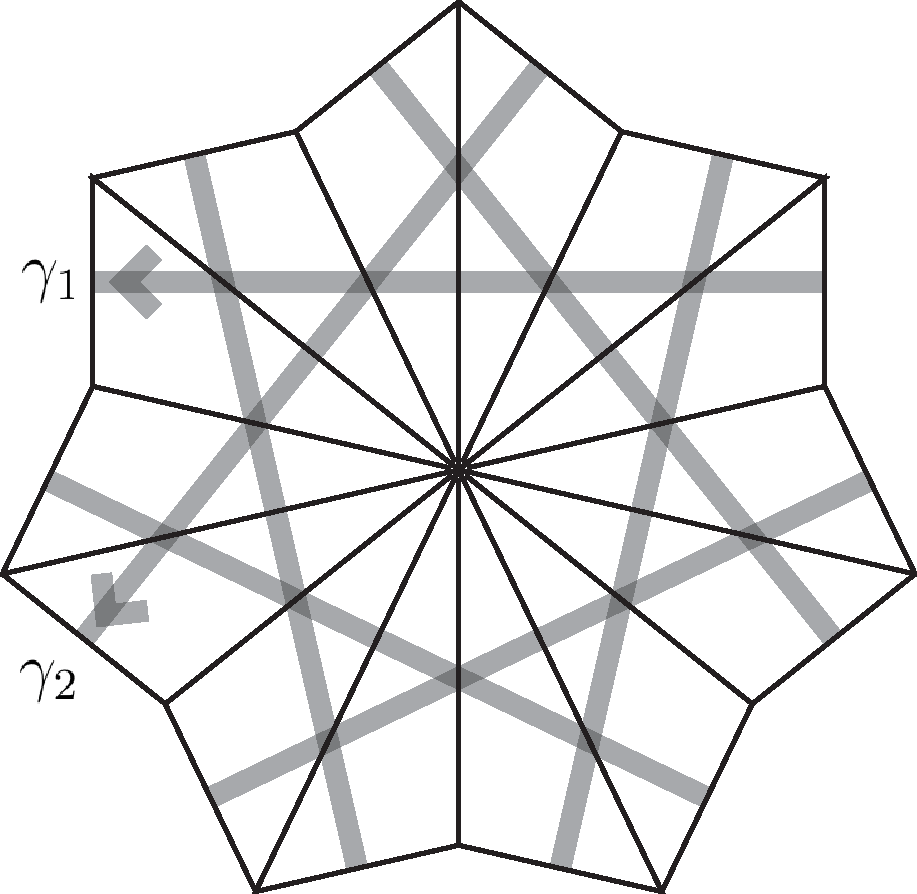
\includegraphics[width=2in]{figures/124_flat} 
	\caption{The flat fourteengon represents $\omega_1$}
	\label{fig: 124_flat}
\end{figure}

The identification of edges are via parallel translations, which verifies that the cone metric is admissible. Identification of parallel edges yields closed cycles and the cyclicity gives away a homology basis with the following intersection matrix

$$\textrm{int} = \begin{pmatrix}
 0 & 1 & 1 & 0 & 0 & -1 \\
 -1 & 0 & 1 & 1 & 0 & 0 \\
 -1 & -1 & 0 & 1 & 1 & 0 \\
 0 & -1 & -1 & 0 & 1 & 1 \\
 0 & 0 & -1 & -1 & 0 & 1 \\
 1 & 0 & 0 & -1 & -1 & 0 
\end{pmatrix}.$$

Furthermore, we can produce flat structures that arise from $\omega_2$ and $\omega_3$ which are achieved from multipliers. The following period matrix is computed using the method from \cite{kw}.

 $$(\Pi) = (\int_{\gamma} \omega) = \begin{pmatrix}
  1 & \zeta  & \zeta^2 & \zeta^3 & \zeta^4 & \zeta^5 \\
 1 & \zeta^2 & \zeta^4 & \zeta^6 & \zeta^8 & \zeta^{10} \\
 1 & \zeta^4 & \zeta^8 & \zeta^{12} & \zeta^{16} & \zeta^{20} 
 \end{pmatrix}$$ where $\zeta$ is the seventh root of unity.


\subsection{Exhibiting the Automorphism Group via Tessellation}

\label{sec:flagflag}

In \cite{dami}, the first author computed the automorphism group of an eightfold cyclic cover over a thrice punctured sphere by finding a tessellation on the surface where the vertices corresponded to the Weierstrass points. There, the surface of interest has Weierstrass points of uniform weight. In this paper, we conjecturally generalize this algorithm to surfaces that have Weierstrass points of different weights. %We will use Weierstrass points, computed using the Wronski metric, as our markings on the surface.

In this section, we wish to find a tessellation $\Delta$ on a surface $S$ which exhibits the automorphism group of $S$. Formally, we wish for $\Aut(S)$ to act freely and transitively on the tiles of $\Delta$; we denote this with a slight abuse of notation:
\vspace{-3pt}
$$\Aut(\Delta) \simeq \Aut(S)$$

This notation is partially justified by defining $\Aut(\Delta)$ to be the group of automorphisms which are orientation-preserving, send vertices to vertices, edges to edges, and faces to faces. 

\begin{defn} A \textbf{tessellation} $\Delta$ is a polygonal decomposition of the surface where the polygons are either disjoint or share an edge or vertex, and their union is the entire surface. We say $\Delta'$ is a refinement of $\Delta$ if $\Delta \subset \Delta'$. \end{defn}

\begin{defn} \label{defn: base tess} Let $S$ be a $d$-fold cyclic cover over an $n$-punctured sphere. We define the \textbf{base tessellation} of $S$ as a tessellation tiled by $n$-gons with valency $d$ at every vertex. \end{defn}

%\begin{defn} An \textbf{all-seeing tessellation} on a surface $S$ is such that $$\Aut(\DD) \simeq \Aut(S) $$ \end{defn}

%We wish to construct an all-seeing tessellation for any given cyclically branched cover $S$ of a sphere. Our first step is the base tessellation.
\textbf{Algorithm:} A particular tessellation $\Delta_T$ on $S$.


%%%lookd: A tessellation $\Delta_T$ on $S$ such that all tiles are similar, all Weierstrass points occur as vertices, and (the fundamental domain condition is hard to state nicely?)


\textit{Input:} A surface $S$ which is a cyclically branched cover of a sphere. \n
$\text{}$ $\hspace{2mm}$\textit{Output:} A particular tessellation $\Delta_T$. 
\begin{enumerate}
\item  Construct a base-tessellation $\Delta$ of $S$.
\item Separately, find the Weierstrass points of $S$ using Definition~\ref{def: wronski}. 
\item Refine $\Delta$ until all tiles are similar and all Weierstrass points of $S$ occur as vertices. Call this new tessellation $\widetilde{\Delta}$. 

%Attempt to align the Weierstrass points of $S$ with the vertices of $\Delta$. If this is not possible, refine $\Delta$ until all Weierstrass points lay on vertices of $\Delta$ and all tiles of $\Delta$ are similar. Call this new tessellation $\widetilde{Delta}$. 

\item Let $G_T$ be the orientation-preserving automorphism group of a tile $T$ of $\widetilde{\Delta}$ (recall that all tiles are similar\footnote{Note that the automorphism group $G_T$ encodes the weight of the vertices of $T$. As automorphisms preserve weights, vertices of different weights cannot be mapped to each other. Since all $T$ are similar, all $G_T$ are the same.}). Restrict our attention to a tile $T$ of $\widetilde{\Delta}$. On this tile $T$, add lines until any tile of the refinement $T'$ is the fundamental domain of $G_T$ acting on $T$. Doing this to every tile $T$ gives a new tessellation, which we call $\Delta_T$.


%%%lookd: can we have an issue where the rotation of the fundmental domain T' is an automorphism of the surface S?
% so a rotation that fixes a T? This happens but why would it be an issue? For instance, Klein's quartic has 56 order-three rotations. 

\end{enumerate}

\begin{conjecture} \label{tessconj}
The output tessellation $\Delta_T$ of this algorithm always exists and $$\Aut(\Delta_T) \simeq \Aut(S)$$
\end{conjecture}

By checking against the automorphism groups obtained via the \texttt{autplane} program described in Section ~\ref{sec:autplane}, we have shown this conjecture to be true for the cyclically branched surfaces of genus $< 5$ mentioned in Section ~\ref{sec:examples}.


 %We can also prove that it is true for the case where our surface $S$ is in fact a quotient of a periodic polyhedral surface in $\R^3$, e.g. Fermat's curve, Schoen's I-WP Surface, and Bring's curve.

%\ti{lookd: is it true? CHECK THIS! Can we prove this for surfaces which are quotients of polyhedral surfaces? Fermat's, I-WP, and Bring's are still cyclic covers over spheres. I don't know all triply periodic polyhedral surfaces. I have three more examples of tpps that are also cyclic branched covers and I also have examples of tpps that are not cyclic covers over spheres. The latter, I have no info about.}

\begin{example}
We perform an example of this algorithm for Klein's quartic. We begin with the base tessellation Figure~\crefformat{figure}{~#2#1{(a)}#3} \cref{fig:124}. Both $d$ and $n$ play a role as we already know the existence of the $d$-fold map and the order-$n$ map that permutes the branched values. The base tessellation is unique due to the Gauss-Bonnet formula. For example, the base tessellation of Klein's quartic is tiled by hyperbolic $\frac{2 \pi}{7}$-triangles (Figure~\crefformat{figure}{~#2#1{(a)}#3} \cref{fig:124}). Since the genus is three, we have $2 \pi (2 - 2 \cdot 3) = -56 (\pi - 3 \cdot \frac{2 \pi}{7})$ hence we need 56 triangles. Next, we locate all Weierstrass points. On Klein's quartic, all vertices of the base tessellation correspond to Weierstrass points, that is $\Delta = \widetilde{\Delta}$. We move to the last step. Since each tile $T$ of $\widetilde{\Delta}$ is a regular triangle with all vertices the same weight, we get $G_T = \Z/3$. Thus, we add lines to each tile $T$ such that each tile $T'$ is now a fundamental domain for the action of $G_T$ on $T$. (Figure~\crefformat{figure}{~#2#1{(b)}#3} \cref{fig:124}).

%%%lookd: if this is Z/3, why are there 6 tiles in T'
% this includes orientation-reversing ones. If it makes more sense, I will remove these lines.

 \end{example}


%\footnote{For example, if the tile $T$ is a regular triangle with all 3 vertices the same weight, it has symmetry group $\Z/3$.}


%However, if not all Weierstrass points are located at the vertices of the base tessellation, we subdivide the tiles so that Weierstrass points are at the vertices.

%We claim that the smallest tile we achieve represents $\Aut(S).$

\begin{figure}[htbp]
    \centering
    \subfloat[The base tessellation $\Delta$]{{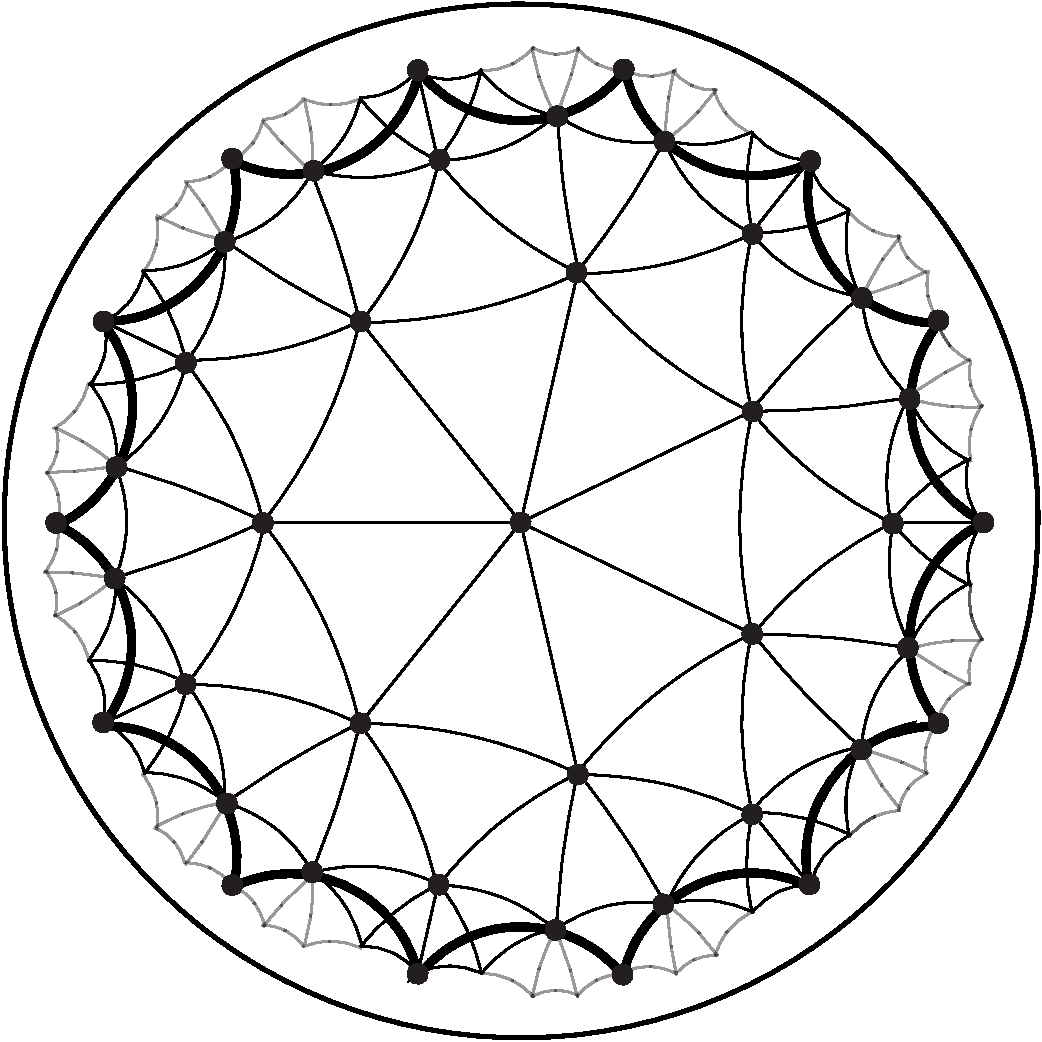
\includegraphics[width=2.75in]{figures/124_base}}}
    \qquad
    \subfloat[The refined tessellation $\Delta_T$]{{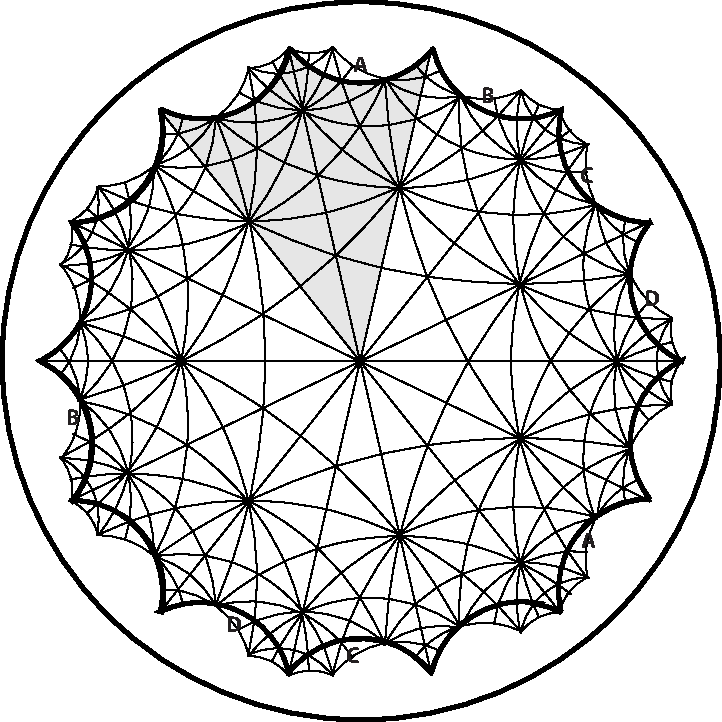
\includegraphics[width=2.75in]{figures/124_hyp}}}%
    \caption{Klein's quartic}%
    \label{fig:124}%
\end{figure}

A Weierstrass point on a non-singular irreducible algebraic curve $S$ is a point $P$ for which there exist functions on the curve with unusual pole orders at $P$ and no poles everywhere else. Hurwitz showed that if the genus $g$ is greater than 2, there there do exist Weierstrass points, and the number of Weierstrass points is bounded by $2g+2 \leq \omega \leq g(g+1)(g-1)$. Further, when genus $g \geq 2$, then $\Aut(S)$ is finite.  In characteristic zero, this can be proved by showing that every automorphism fixing more than $2g + 2$ points is the identity (by the Riemann-Roch theorem), and then obtaining a faithful representation of $\Aut(S)$ as permutations of the set of Weierstrass points $L: \text{Aut}(S) \to \Sigma_\omega$. Note that in general, the action of $\Aut(S)$ on the set of Weierstrass points is not transitive.

We calculate the Weierstrass points of a surface by finding the zeros of the Wronskian.
\begin{defn} Given a basis of holomorphic functions $\{f_1, \ldots , f_g\}$ on a Riemann surface $X$ of genus $g$, the Wronskian defined by $$\mathcal{W}(z) := \textrm{det} \left( \frac{d^j f_k(z)}{d z^j} \right)_{j = 0, \ldots , g - 1, \, k = 1, \ldots , g}$$ is a non-trivial holomorphic function on $X$ that induces a metric which we call the \textit{Wronski metric.} 
\end{defn}


%In general, we find all-seeing tessellations on such surfaces $S$ using prior knowledge of the automorphism group of $S$. 

%the vertices are coming from the punctures in the underlying sphere, and the tesselation is a lift of the tesselation of the underling sphere (where we choose some special metric on the underlying sphere coming from Gauss Bonnet on the cyclic cover S?) 
%Is this correct?
%when you said "the special cases where we know the polyhedral tiling" do you mean we know those surfaces are quotients of polyhedral surfaces in R^3? 

%In some special cases, we know that our surface $S$ is in fact a quotient of a periodic polyhedral surface in $\R^3$, e.g. Fermat's curve, Schoen's I-WP Surface, and Bring's curve. In these very special cases, we can construct an all-seeing tessellation on $S$ without knowing the automorphism group of $S$ a priori. Thus, we can compute the automorphism group of $S$ from the all-seeing tessellation. \ti{prove that we can do it in the case of a quotient of a periodic polyhedral surface quotients?}

%\ti{Add some background here, define weierstrass points, mention Riemann roch, that it is a very rare property for the group to act transitively on the Weierstrass points, wronski to find them}
% Weierstrass points and Wronski are defined in section 2.1. Riemann-Roch is briefly mentioned there too.


\section{The Precise Torelli Theorem}
\label{sec:torelli}


\begin{remark} The first portion of this section is an English translation of the first two paragraphs of the Appendice \cite{Torelli}, with slight modifications for the reader's convenience.\end{remark}

Let $k$ be a field, and let $X_{/k}$ be a nice (smooth, projective and geometrically integral) curve over $k$ of genus $g > 1$.  Let $(\operatorname{Jac}(X),a)$ denote the Jacobian of $X$ together with the Jacobian's canonical principal polarization $a$, which is of degree 1.  Let $X'_{/k}$ be another nice curve. Any isomorphism $f: X \to X'$ defines by functoriality an isomorphism $f_J: (J, a) \to (J', a')$. 

\begin{remark} The isomorphism $f: X \to X'$ induces an isomorphism between $\text{Div}^i(X)$ and $\text{Div}^i(X')$ for every $i$. This is because $Div$ is defined as formal combinations of codimension 1 subvarieties, and we can pull the inclusions of subvarieties of $X'$ into $X$ back via the isomorphism $f$. Note that the image of $\text{Div}^{g-1}(X)$ under the Abel-Jacobi map determines the canonical principal polarization of $\Jac(X)$ with respect to $X$. \end{remark}

%\begin{remark} This functoriality can more easily be seen when we consider that $Pic^0(X)$ is dual to $Jac(X)$, then the induced map from $f: X \to X'$ is just the pullback of line bundles $f^*: Pic^0(X') \to Pic^0(X)$, and further, considering the principal    \end{remark}
 

%defines by structure transport an isomorphism $f_J: (J, a) \to (J', a')$. 

Torelli's theorem says that we get almost all of the isomorphisms: $(J, a) \to (J', a')$. More precisely:

\begin{thm*} Suppose $X$ is hyperelliptic.  Then for every isomorphism of polarized abelian varieties $F: (\operatorname{Jac}(X),a) \stackrel{\sim}{\rightarrow} (\operatorname{Jac}(X'),a')$, there exists a unique isomorphism $f: X \stackrel{\sim}{\rightarrow} X'$ such that $F = \operatorname{Jac} f$.  \end{thm*}

\begin{thm*} Suppose $X$ is not hyperelliptic.  Then, for every isomorphism of polarized varieties $F: (\operatorname{Jac}(X),a) \stackrel{\sim}{\rightarrow} (\operatorname{Jac}(X'),a'),$ there exists an isomorphism $f: X \stackrel{\sim}{\rightarrow} X'$ and $e \in \{ \pm 1\}$ such that $F = e \cdot  \operatorname{Jac} f$.  Moreover, the pair $(f,e)$ is uniquely determined by $F$. \end{thm*}

So, we conclude: 

$$\Aut(\Jac(X), a) \simeq \begin{cases} \Aut(X) & \text{if } X \text{ is hyperelliptic} \\
\Aut(X) \oplus \Z/2 &  \text{if } X \text{ is not hyperelliptic}
\end{cases} $$

%\begin{remark} There is a very important point here. $\Aut(X)$  is \textit{not} the pointed automorphisms. Indeed, the pointed automorphism groups \textit{depend on the choice of point}. \end{remark}

%page 203 Jacobian Varieties Cornell-Silverman: Arithmetic Geometry

%Serre states this as a ``precise" form of the Torrelli theorem, and further, that no proof of it is in its entirety is in the literature as far as he knows.  
(Here we end quoting the Appendice). This precise form of Torelli's theorem is proved for algebraically closed fields by Weil \cite{oe}. A modern proof by Martens \cite{finn} proves Torelli's theorem as a combinatorial consequence of the Riemann-Roch theorem and Abel's theorem. Let $\phi$ be the Abel-Jacobi map $\phi: X \to \Jac(X)$ (this map is determined up to translation by the torus $\Jac(X)$). Let $\Div^i(X)$ denote the degree $\leq i$ effective divisors on $X$, and $W^i$ denote their image $\phi(\Div^i(X))$. 


%\ti{clean up the following or take it out, how does this move the tessellation of the embedded X into Jac(X)  (Visualizing the induced tessellation on the Jacobian)}

Note that: 

\begin{itemize} 
\item $\Div^1(X)$ is simply the points on $X$, so  $\Div^1(X) = X$.

\item $W^1$ is birationally equivalent to $X$, that is, we can think of $X$ as being embedded in its Jacobian. 

\item  $W^{g-1}$ determines the canonical polarization of $\Jac(X) = W^g$ with respect to $X$.  

\item There is a map \begin{align*}
\text{flip}: \Jac(X) &\to \Jac(X)\\
u &\mapsto -u + \phi(Z)
\end{align*}
where $Z$ is a canonical divisor on $X$.
\item By translation of $U$, we mean for every $p \in U \subset \Jac(X),$ we have $p+a$ using the Jacobian group operation.
\end{itemize} 

Let $Y$ and $X$ have the same Jacobian, and $V^{k}$ denote $\phi(\Div^k(Y))$. We finish by showing that if the canonical polarizations are the same, i.e. $V^{g-1} = W^{g-1}$, then $V^1$ is a translate of $W^1$ or $\text{flip}(W^1)$. This is done by induction on the smallest $r$ such that $V^1 \subseteq W^{r+1}$ or $V^1 \subseteq \text{flip}(W^{r+1})$, up to translation, showing that $r$ must be 0.

%Taking into account the tessellation-flag method of computation of the automorphism groups of Riemann surfaces (which are cyclic covers of the sphere), we may visualize this as inducing a tessellation on the Jacobian via the tessellation on the embedded variety.\ti{clarify this}

 In the case of hyperelliptic curves, $W^1 = \text{flip}(W^1)$, that is, they coincide as sets in $\Jac(X)$. For non-hyperelliptic curves, $W^1 \neq \text{flip}(W^1)$, hence the $\Z/2$ factor. 




%add the divisor theoretic statement of Weil. 

\begin{comment}

The proof summary is translated from German by the second author (using the above notation of Serre).

[Let $\Theta$ be the underlying manifold of the Jacobian $J$. ?? Or is it a divisor?]

``The proof is given by this: that one specifies an explicit construction of $C$ and $\phi$ [(the canonical map from $C \to Jac(C)$)] (when?) one already knows the Jacobian (??).

First, it will be shown that the collection $\{\Theta_a\}$ of manifolds resulting from $\Theta$ by translation are uniquely determined by the polarization of $J$. In the classical case, this follows from known theorems in the theory of theta functions. In the abstract case, this follows from the following sentence:

[the divisor theoretic statement]

"


\end{comment}

%\begin{theorem} ``Let $C, C'$ be two curves of the same genus $g > 1$; let $\phi$ (resp. $\phi'$) be the canonical maps from $C$ (resp. $C'$) to their Jacobians $J$ (resp. $J'$). Let $\phi: Jac(J, \phi) \stackrel{\sim}{\rightarrow} Jac(J', \phi')$. Then, this gives us an isomorphism $f: C \stackrel{\sim}{\rightarrow} C'$ with the property that $\alpha \circ \phi  = \pm \phi' \circ f + a$ is with constant $a$; while $f$, $a$, and the sign $\pm$ are uniquely determined by $\alpha$, if $C$ and $C'$ are not hyperelliptic; while $C$ and $C'$ are hyperelliptic, $f$ and $\phi$ are by $\alpha$ uniquely determined, and the sign can be chosen arbitrarily [literally: any sign can be chosen]?  \end{theorem}

%\todo[inline]{add a proof summary here to help understand where the extra Z/2 is coming from -- why determined up to translation and reflection?? how can we view this tessellation change explicitly?}

%https://www.jstor.org/stable/1970505?seq=1#page_scan_tab_contents


 


%might be worth it to go through the proof and try to restructure it into something readable. 


%\cite{oe}

%Oeuvres Scientifiques - Collected Papers II, [1957a], Zum Beweis des Torellischen Satzes, Sektion 2: Hauptsatz



%\begin{remark} This can either be seen as leading us to a very subtle point on the relation between a curve and its Jacobian, exposited by \cite{yifeng}. Or, we can see it as an analogue of the James construction -- where a point must be chosen but in the end the point does not matter. \end{remark}


\section{Programmatically Computing the Automorphism Group of Plane Curves and Abelian Varieties over $\mathbb{C}$}

\begin{remark} This section is copied with from section 4 of Bruin-Sijsling-Zotine \cite{jeroen} with exposition and examples added for the readers' convenience.\end{remark}

Let us examine abelian varieties represented as analytic groups $X := V/\Lambda$ and $X' := V'/\Lambda'$. They need not be Jacobians.

%\begin{remark} We slightly abuse notation here, $\Lambda$ represents both a matrix in $M_{g \times 2g}(\Z)$, and the $2g$-integral-dimensional (i.e., $g$-complex-dimensional) lattice in $\C^g$ generated by the columns of that matrix.\end{remark}
 
%A homomorphism $\phi: J \to J'$ induces a tangent map $V \to V'$ and a map on ``homology"\footnote{In the case of Jacobians $\Jac(C) = H^0(C, \Omega_{C}^1)/H_1(C; \Z) \simeq \C^g/\Lambda$, hence the name homology representation for the map on $\Lambda$.} $\Lambda_1 \to \Lambda_2$. After a choice of basis, these correspond to matrices $T=T_\phi \in M_{g_2 \times g_1}(\C)$ and $R = R_\phi \in M_{2g_2 \times 2g_1}(\Z)$. 

%Let $\Lambda_1 = (A \mid B)$, that is, break the gx2g matrix into two square matrices.



\begin{thm*}[BL 1.2.1] Let $X:= V/\Lambda$ and $X':= V'/\Lambda'$ be abelian varieties. Under addition the set of homomorphisms $\Hom(X, X')$ forms an abelian group. There is an injective homomorphism of abelian groups: 


\begin{align*} 
\rho: \Hom(X, X') &\to \Hom(V, V') \\
f &\mapsto F
\end{align*} 

The restriction to the lattice $\Lambda$ is $\Z$-linear, thus we get an injective homomorphism: 


\begin{align*} 
\rho|_{\Lambda}: \Hom(X, X') &\to \Hom_{\Z}(\Lambda, \Lambda') \\
f &\mapsto F|_{\Lambda}
\end{align*} 


\end{thm*}
%Let $E := \begin{pmatrix} 0 & I \\ -I & 0 \end{pmatrix}$, in other words, the standard symplectic matrix.

We will namely use the representation $\rho|_{\Lambda}$ and find the basis of our set of maps in terms of this representation. 

We work in the category of varieties equipped with principal polarizations, which we discuss in section~\ref{sec:intropol}. In this category, morphisms are morphisms of pairs. That is,

$$f: (X, c_1(\mc{L})) \to (Y, c_1(\mc{M}))$$

such that $f^*(Y, c_1(\mc{M})) = (X, c_1(\mc{L}))$ (for isomorphisms).  We may represent polarizations as integral valued alternating forms. 

% tktk 
% define polarization here before using it in the next definition


\begin{defn} Let $a$ be a polarization of $X$. We call $\Aut(X, a)$ a \textbf{symplectic automorphism group} of $X$, as it respects the symplectic form $a$. 
\end{defn}

% tktk 
% Define/mention what R is here. You use it in the algorithm but there's no info about that here. 

Let $E_1$ and $E_2$ be forms representing $c_1(\mc{L}_1)$ and $c_1(\mc{L}_2)$, respectively. Note that a map $\alpha: (X_1, c_1(\mc{L}_1)) \to (X_2, c_1(\mc{L}_2))$ such that $$\alpha^*(c_1(\mc{L}_2)) = c_1(\mc{L}_1)$$ is equivalent to $R$ in the image of $\rho|_{\Lambda}$ such that $$R^tE_2R = E_1$$


\subsection{Computing the Automorphism Group of Plane Curves}
\label{sec:autplane}

\begin{remark} This section is on the algorithm used in \texttt{autplane.sage}. \end{remark}

In the case that our abelian variety is of the form $\Jac(C_i) =: J_i$, and we know the curve $C_i$, there is a special principal polarization $E_i$ with respect to that curve $C_i$. This is programmatically found using Lemma 2.6 from \cite{jeroen}. 
\vspace{+10pt} 
%The following psuedocode is copied from section 4.2 ``Computing symplectic isomorphisms" \cite{jeroen}  for the readers convienience. Note that steps 4-7 coicide with steps (???) in the previous algorithm, however, since the canonical principal polarizations are known, we use only one iteration of steps 5-7. We write it out to avoid unneccessary confusion.


%or equivalently, $\alpha_*(c_1(\mc{L})) = c_1(\mc{M})$.

\textbf{Algorithm:} Compute the set of isomorphisms between curves. 

\textit{Input:} Planar equations $f_1$, $f_2$ for curves $C_1$, $C_2$.\n
$\text{}$ $\hspace{2mm}$\textit{Output:} The set of isomorphisms $C_1 \to C_2$, or the group $\Aut(C)$ if $C_1 = C_2$.

\begin{enumerate}
\item Check if $g(C_1) = g(C_2)$; if not, return the empty set.
\item Check if $C_1$ and $C_2$ are hyperelliptic; if so, use the methods in \cite{hyp}.
\item Determine the period matrices $P_1, P_2$ of $C_1, C_2$ to the given precision.
\item Determine a $\Z$-basis of $\Hom(J_1, J_2) \subset M_{2g \times 2g}(\Z)$ represented by integral matrices $R \in  M_{2g \times 2g}(\Z)$. [Lemma 4.3 \cite{jeroen}]
\item Using Fincke-Pohst\footnote{This is an algorithm for finding vectors of small norm. We use it here to solve for the finite set of solutions $R = \sum_{i = 1}^{2g} \lambda_i B_i$, where $B$ is the basis from step 4.}, determine the finite set [from 5.1.9 BL] $$S = \{ R \in \Hom(J_1, J_2) \text{ } | \text{ } \text{tr}((E_1^{-1}R^tE_2)R) = 2g\}$$
\item Return the subset\footnote{The condition $R^tE_2R = E_1$ (i.e., $E_1^{-1}R^tE_2R = \text{Id}$) implies that $\text{tr}((E_1^{-1}R^tE_2)R) = 2g$. So we first solve for the latter to thin the results, then solve for the former from that set.}  of $R \in S$ which further satisfies $R^tE_2R = E_1$. (These are the symplectic endomorphisms.)
\item Look at the subset of $R$ such that $\det(R) = \pm 1$. These are the symplectic automorphisms.
\item If $J_1 = J_2$, find the group structure of this subset.
%Using the canonical morphisms with respect to the chosen basis of differentials, return the subset of elements of $S$ that indeed induce an isomorphism $J_1 \to J_2$.
\end{enumerate}

\vspace{+10pt} 

Note that if the curves $C_1$ and $C_2$ are non-hyperelliptic, by the precise Torelli theorem, we get $\Hom((J_1, E_1), (J_2, E_2)) \simeq \Hom(C_1, C_2) \sqcup \{ \pm 1 \}$ from this algorithm. So, we must remove the direct summand $\{ \pm 1 \}$.

\begin{remark} Step 8 of the above algorithm was added by the second author to tame these unwieldy matrix groups, and is achieved as follows.\end{remark}

\textbf{Algorithm:} Compute the group structure of an underlying set of matrices.

\textit{Input:} A set of matrices which are a group by multiplication. \n $\text{}$ $\hspace{2mm}$\textit{Output:} The group structure of the set.

\begin{enumerate}
\item Check cardinality of the set. Call this $N$.
\item Take first 15 elements of the set, use GAP to check if these generate a matrix group $G$ of the correct order $N$. If not, it generates a group of order $K$, where $KM = N$. Take more elements of order dividing $M$ until they generate a group of the correct order.
\item Use \texttt{IdGroup(G)} in GAP.
\end{enumerate}



%how is frobenius form like elementary divisors for alternating integer matrices.?

\subsection{Computing the Automorphism Group of Abelian Varieties}
\label{sec:autperio}

\begin{remark} This section is on the algorithm used in \texttt{autperio.sage} \end{remark}

\begin{notation} Let $A:= V/\Lambda$ be an abelian variety of dimension $g$. Let $e_1, ..., e_g$ be the chosen basis for $V$, and $\lambda_1, ..., \lambda_{2g}$ be a corresponding chosen basis for $\Lambda$. Let $\Pi$ be the corresponding period matrix such that $A := \C^g/\Pi \Z^{2g}$.
\end{notation}

\textbf{Algorithm:} Compute the group of isomorphisms between abelian varieties. 

%what makes these automorphisms symplectic? 

\textit{Input:} Period matrices of abelian varieties $J_1$ and $J_2$, as $\Pi_1$ and $\Pi_2$ respectively. \n
$\text{}$ $\hspace{2mm}$\textit{Output:} For each combination of principal polarizations $(a_i, b_j)$, the set of isomorphisms between $(J_1, a_i)$ and $(J_2, b_j)$ (or the group, if they coincide).
\begin{enumerate}
\item Check if $g_1 = g_2$; if not, return the empty set.
\item Determine a $\Z$-basis of $\Hom(J_1, J_2) \subset M_{2g \times 2g}(\Z)$ represented by integral matrices $R \in  M_{2g \times 2g}(\Z)$.
\item Find many principal polarizations $\{a_i\}$ and $\{b_j\}$ for $J_1$ and $J_2$ respectively using \texttt{CullPB} (exposited in the next section).
\item Apply steps 5-8 of the previous section substituting each pair $(a_i, b_j)$ for $(E_1, E_2)$. For each pair, this will produce the set of isomorphisms between $(J_1, a_i)$ and $(J_2, b_j)$.
\item If $(J_1, a_i) = (J_2, b_i)$, find the group structure of each set $\Aut(J_1, a_i)$ (using the algorithm in the previous section).
\end{enumerate}

%what makes these automorphisms symplectic? 



%\begin{remark} This algorithm is a repeat of the algorithm in the next section, beginning with different inputs [it begins at step (4) of the algorithm for plane curves]. We exposit it seperately to emphasize that is works for more than just plane curves. \end{remark}




%In the following description of the program, we assume that the period matrix is already known. We find the period matrix using either Lee-Webers's method for cyclic covers \todo{does it work more generally?}, or using Bruin's calculation of the period matrix from the Voronoi cell decomposition.

\subsection{Introduction to Polarizations: From Theory to Code}
\label{sec:intropol}
The notion of a polarization of an abelian variety has many faces. If a complex torus has a polarization, it is an abelian variety.

\begin{defn} A \textbf{polarization} of a complex torus $X$ is an embedding $j: X \to \P^N$ for large enough $N$. \end{defn}


%is it important that it is a projective embedding

We can understand this embedding $j$ as a map $$p \mapsto [a_1(p) : \cdots : a_{N-1}(p)]$$ where $a_i$ are a chosen generating set of global sections of a line bundle $\mc{L}$ on $X$. 

%locally free of rank 1 globally generated sheaf = ample line bundle; are other ranked globally generated sheaves going to give other embeddings? 

\begin{defn} A line bundle $\mc{L}$ is defined to be \textbf{very ample} on $X$ if it defines a closed embedding into $\P^N$ for large enough $N$. %if it has finitely many global sections, such that for every $x \in X$, there is at least one section not vanishing at this point. 
\end{defn}

\begin{defn} A line bundle is \textbf{ample} if a tensor power of the line bundle is very ample. Since the Chern class is additive, $c_1(\mc{L}^{\otimes k}) = kc_1(\mc{L})$, the ample bundle and its tensor power are equivalent datum. \end{defn} 

\begin{remark} In other words, $\mc{L}$ is defined to be ample if it (or a tensor power of it) specifies an embedding of $X$ into projective space.\end{remark}

%Note that $\mc{F}$ is a sheaf generated by its finitely many global sections. We may restate this property as follows. 

%\begin{remark} Let $X$ be a Riemann surface of genus $g$. We can understand this embedding $j$ as the map $$p \to [\omega_1(p) : \cdots \omega_g(p)]$$ where $\omega_i$ are a chosen basis of holomophic differentials on $X$, that is, a chosen generating set of global sections of a line bundle (the sheaf of differential 1-forms). This is where we get the canonical polarization associated to a curve. \end{remark}
%This embedding information is often specified by \todo[inline]{IS IT EQUIVALENT TO} an ample line bundle $\mc{L}$ on $X$. 

\begin{defn} Line bundles $\mc{L}_1$ and $\mc{L}_2$  on $X$ are \textbf{analytically equivalent} if there is a connected complex analytic space $T$, a line bundle $\mc{L}$ on $X \times T$, and points $t_1, t_2 \in T$ such that $$\mc{L} |_{X\times \{t_i\}} \simeq \mc{L}_i$$ for $i = 1, 2$. \end{defn}

A line bundle $\mc{L}$ over $X$ is specified up to analytic equivalence by its first Chern class $c_1(\mc{L}) \in H^2(X; \Z)$. More precisely,

\begin{thm*} 
[2.5.3 BL] Let $X$ be an abelian variety. For line bundles $\mc{L}_1$ and $\mc{L}_2$ over $X$, the following statements are equivalent: 
\begin{enumerate} 
\item $\mc{L}_1$ and $\mc{L}_2$ are analytically equivalent.
%\item $\mc{L}_1 \otimes \mc{L}_2^{-1} \in \text{Pic}^0(X)$
\item $c_1(\mc{L}_1) = c_1(\mc{L}_2)$
%\item $\phi_{\mc{L}_1} = \phi_{\mc{L}_2}$
\end{enumerate}
\end{thm*}


%We may recover a line bundle $\mc{L}$ on $X$ from its first chern class by $(f, c_1(\mc{L}))^*(\mc{P}_X) \simeq \mc{L}^{\otimes 2}$, where $\mc{P}_X$ is the Poincare correspondence on $X$.  


%and a semi-character $\chi$.  \ti{add more on semicharacter, is it needed to fully specify polarization}


\begin{defn} The \textbf{first Chern class} of a line bundle $\mc{L}$ is the image of $\mc{L} \in \Pic(X) = H^1(\mc{O}_X^*)$ under the map $c_1$ on cohomology which arises as follows. Consider the exact sequence $$0 \to \Z \to \mc{O}_X \to \mc{O}_X^* \to 0$$ and its long cohomology sequence:
%\to H^1(X, \Z) \to H^1(\mc{O}_X) \to 
$$\cdots \to H^1(\mc{O}_X^*) \xrightarrow{c_1} H^2(X, \Z) \to \cdots$$ \end{defn} 

%\ti{is there a more universal defn?} 


%pp works for all varieties, why are algebraic varieties abelian?

%\ti{why is chern class of line bundle automatically integral by [BL B.1 and 2.1.1]?}, because that is its target!!!

%By definition, every (chern class of a holomorphic) line bundle on $X$ \in H^2(X, \Z)

We associate to every first Chern class an alternating form.

\begin{thm*} [BL 1.3.2 \& 2.1.2] $$\psi: H^2(X; \Z) \simeq \Alt^2(\Lambda, \Z)$$ 
\end{thm*} 



%To each element of $S$, 

%This associates to every (chern class of a holomorphic) line bundle on $X$  
%\ti{explore this because the code in 4.4 doesn't seem to reflect this, what small combinations is CullPB using to check if it has det 1?? how is CullPB checking thm 10?} 
 
 
Let $S$ be the set of $c_1(\mc{L})$ where $\mc{L}$ ranges over all holomorphic line bundles on $X$. The image $\psi(S)$ is isomorphic to all Hermitian alternating forms.

%\begin{remark} We may use the Frobenius form to calculate all Hermitian forms and prune out those which are in $\phi(S)$. \end{remark}


%It is specifically the Hermitian forms which come from line bundles represented as maps $X \to \hat{X}$ (this representation is explained in section???).

\begin{thm*} [BL 2.1.6] Let $X:= V/\Lambda$ be an abelian variety. For an alternating form $E: V \times V \to \R$, the following conditions are equivalent: 

\begin{enumerate} 
\item There is a holomorphic line bundle $\mc{L}$ on $X$ such that $\psi(c_1(\mc{L}))= E$. 
\item $E(\Lambda, \Lambda) \subseteq \Z$, and $$E(iv, iw) = E(v, w)$$
\end{enumerate}
\end{thm*} 

 
\begin{remark} Note that from each element $\Alt^2(\Lambda, \Z)$ we obtain via $\R$-linear extension an alternating form $\Alt^2(V, \R)$ (as in rational versus analytic representation, see [BL 1.2.1]). We also have an isomorphism between real valued forms satisfying 2.1.6(2) and Hermitian forms. \end{remark}

It is important to emphasize that not all forms satisfying 2.1.6(2) correspond to Chern classes of ample line bundles. Ampleness is stronger than holomorphicity, hence we need a stronger condition. 

\begin{defn} 
A line bundle $\mc{L}$ on $X$ is called \textbf{positive} if $c_1(\mc{L})$ is represented by a positive-definite Hermitian form.
\end{defn}

\begin{thm*} 
Let $X$ be a smooth complex projective variety. A line bundle $\mc{L}$ on $X$ is ample if and only if it is positive.
\end{thm*}

%We end our descent from theory to practice with the test for how to check if an alternating integral form is Hermitian.

%\begin{remark} By [BL 2.1.7], the alternating forms over $\R$ of 2.1.6 are the imaginary parts of hermitian forms over $\C$. That is, there is a bijection between the set of Hermitian forms on $V$ and the set of real valued alternating forms on $V$ satisfying $E(iv, iw) = E(v, w)$. \end{remark} 

This is how we ask the computer to find polarizations of an abelian variety $X$, which are steps 1 and 2 of the following section.

However, there may be infinitely many polarizations. We are interested in a particular kind of polarization.

\begin{defn}  A polarization $c_1(\mc{L})$ of $X$ is called \textbf{principal} if $\mc{L}$ has only one section up to constants, i.e. $\dim H^0(X, \mc{L}) = 1$.  \end{defn} 

As a motivational theorem:

\begin{thm*} [BL 4.1.2] Every polarization is induced by a principal polarization via an isogeny. \end{thm*}

By Narasimhan-Nori \cite{nn}, there are only finitely many principal polarizations on a variety $X,$ which is irreducible and smooth. And as a corollary, only finitely many curves may have the same Jacobian since each non-isomorphic curve gives a non-isomorphic principal polarization on its Jacobian.


\begin{comment}
\begin{defn} 
The \textbf{Jacobian} of a genus $g$ curve $C$ is defined as quotient space $V/\Lambda$. Here $V$ is the dual of the $g$-complex dimensional vector space of global holomorphic differentials on $C$, i.e. $H^0(C, \Omega_{C/\C}^1) \simeq H^1(C, \mc{O}_C)$, and $\Lambda$ is the lattice of all elements of $V$ of the form $[\gamma]: \omega \mapsto \int_{\gamma} \omega$, where $\gamma$ is a closed curve in $C$. In other words, $\Jac{C} := H^0(C, \Omega_{C, \C}^1)^*/H_1(C)$.
\end{defn} 

\begin{remark} The Jacobian is an ``abelianization" functor from $\Jac: \text{RiemSurf} \to \text{AbVar}_{\C}$. \end{remark}

A curve gives a principal polarization on its Jacobian as follows. We are given an intersection form which takes $\cap: H_1(X, \Z) \times H_1(X, \Z) \to \Z$ (computing the intersection number of two given cycles). 

\begin{remark} We may pick a \end{remark}

We may construct a form $H: H^{1, 0}(C, \C) \times H^{1, 0}(C, \C) \to \Z$ by precomposing $\cap$ with a dualizing map. That is, $H$ takes a pair of forms, returns the dual of each form as a cycle, and computes the intersection of these cycles using $\cap$. By the earlier discussed [BL 2.1.6], this Hermitian form gives a polarization. 

\begin{remark} It is difficult to recover the line bundle corresponding $\mc{L}$ to this polarization $c_1(\mc{L})$ as the inverse to the first Chern class map is very difficult to construct.\end{remark}

\end{comment}

\subsection{Finding Principal Polarizations} 
\label{sec:find}
We begin with a representation of our abelian variety as $A := \C^g/\Pi\Z^{2g}$. 

Then $\Lambda$ is the associated lattice spanned by the columns of $\Pi$. Thus, we have a distinguished basis for the homology of $A$, corresponding to the columns of $\Pi$. 

%\todo[inline]{Do I want to elaborate on this? This is a program, and in a program, we must pick a basis.}

\vspace{+5pt}

\textbf{Algorithm:} Compute many principal polarizations on a given abelian variety $A$.

\textit{Input:} An abelian variety $A := \C^g/\Pi\Z^{2g}$, where $\Lambda$ is the associated lattice to the period matrix $\Pi$. \n
$\text{}$ $\hspace{2mm}$\textit{Output:} Many principal polarizations on $A$.
\begin{enumerate} 

\item The magma function \texttt{FindPolarizationBasis} determines all integral alternating pairings $E$ on the homology, i.e., $E\in \Alt^2(\C^g, \Z)$, for whose real extension we have:

$$E (i v, i w) = E (v, w)$$
This is a basis of alternating forms $\{E_i\}$.
\item Check that $E$ is positive-definite.
\item \texttt{CullPB.m} tries some small combinations and sees if $E_i$ actually gives a pairing with determinant 1 indicating that $E_i$ is a principal polarization. If so, it returns $E_i$. This gives us a set $\{E_k\}$ of integral pairings on the homology.
\item For each $i$, we rewrite these pairings in a symplectic basis. That is, we find a basis of $\Lambda$ in which $$E_i = \begin{pmatrix} 0 & D \\ -D & 0 \end{pmatrix}$$ where $D = \text{diag}(d_1, ..., d_g)$ which we may do by the elementary divisor theorem (section 3.1, \cite{bl}). 

\end{enumerate} 

\begin{remark} This does nothing but modify the (homology) basis of $\Lambda$. Multiplying $\Pi$ on the right with this integral matrix, we get a new period matrix $Q$ whose columns span exactly the same lattice but for which the standard symplectic pairing $E$ is actually the Chern class of a line bundle. This is often called the Frobenius form of the period matrix $\Pi$. \end{remark}


%\footnote{Note that every period matrix $\Pi$ may be written as $(\tau \mid Id)$ where $\tau$ is symmetric with positive definite imaginary part.} We then normalize the left part of $Q$ to be 1. This gives us $\tau$. What do we use tau for then?



%\item As a last step, we check that things (?? do we in fact do this earlier?) are positive definite, to make sure that the aforementioned line bundle is ample.


\begin{defn} We say two principal polarizations $p_1$ and $p_2$ on $A$ are \textbf{auto-equivalent} if and only if $\Aut(A, p_1) \simeq \Aut(A, p_2)$. \end{defn}

This program produces many auto-equivalent principal polarizations. When this equivalent relation is taken, it greatly reduces the number of principal polarizations. Note that auto-equivalence is a weaker notion of equivalence than analytic equivalence, as discussed in section ~\ref{sec:questions}. 

If the abelian variety is indeed a Jacobian, this method will in practice return at least enough polarizations to find the canonical principal polarization. It is an unsolved problem to find all possible principal polarizations associated to a given abelian variety, called ``explicit Narasimhan-Nori". 

\subsection{Abelian Varieties with Several Principal Polarizations}
\label{sec:accident}
An unexpected result of this paper was finding multiple non-autoequivalent principal polarizations on many different Jacobians using a method not found in the literature. Before we state our result we summarize what is known about abelian varieties with several principal polarizations.

\begin{defn} An abelian variety is \textbf{simple} if it is not isogenous to a product of abelian varieties of lower dimension. \end{defn}

Some previous work on finding multiple principal polarizations on abelian varieties has been done by finding two non-isomorphic curves with the same (unpolarized) Jacobian. Therefore, their associated canonical polarizations must be different by the Torelli theorem. Otherwise, the curves would be isomorphic. There are papers which discuss the non-simple case at genus two \cite{iko} and three [Brock, \textit{Superspecial curves of genera two and three}], though the authors was unable to find a copy of the latter. 

\begin{remark} There is only a canonical principal polarization on $A$ if a curve $C$ is specified so that $A = \Jac(C).$ In other words, knowing that $A$ is in the image of the functor $\Jac$ is not enough. \end{remark}

Another technique is used in \cite{howe1} and \cite{howe2} by E. Howe which gives examples of genus two curves that are non-isomorphic but give the same (simple) Jacobian. He does this in characteristic $p$ by playing with isogeny classes of abelian varieties which correspond to special Weil numbers. In \cite{several} Theorem 1.5, Lange establishes that the order of $\Aut(A)$ with certain restriction conditions and equivalence relations is equal to the number of principal polarizations on $A$ up to isomorphism, $\pi(A)$. This bijection between sets is induced by a principal polarization, so one must know that one exists to implement this theorem. One could compute the size of this specially carved out version of $\Aut(A)$ by hand using Lange's theorem. However, we compute directly the principal polarizations on $A$ with the aid of a computer.

%\begin{remark} In Theorem 3.1, Lange further establishes bounds on $\pi(A)$ in terms of the class group of $End_{\Q}(A)$, if $End_{\Q}(A)$ is a \textit{totally real} number field $K$ (and thus the variety $A$ is simple). Since every abelian variety is isogenous to a product of simple abelian varieties $$A \simeq A_1 \times ... \times A_k$$, it is reasonable to ask how the number of principal polarizations on the simple pieces $A_i$ are related to the whole $A$.  \end{remark}  

%More specifically: He does this by considering an element in the Neron-Severi group of $A$, and representing such elements as endomorphisms of $A$ preserved under the Rosati involution with respect to a chosen polarization.   

%First, some notation for Lange's theorem. Let $K$ be a totally real number field of degree $g$ over $\mathbb{Q}$, and let $\mathfrak{o}$ be its principal order. Let $U$ denote the group of units, $P$ the group of principal ideals, $I$ the group of ideals, and $C=I/P$ the class group of $K$ . If $G$ is any of these groups, we denote by $G^+$ the subgroup of totally positive elements. 

%what the hell are totally positive elements? 

%\begin{thm*}[Lange \cite{several}]  \end{thm*} 

%\ti{is the splitting of I-WP nonisomorphic ellitpic curves?} for langes case can we just multiply the bound on the simple cases together?

We use an entirely different technique, exposited in Section ~\ref{sec:find}, which treats both simple and non-simple cases. This technique, for example, gives us 10 not auto-equivalent principal polarizations on the Jacobian of Schoen's I-WP Surface. This is a very interesting result, especially since the variety $\Jac(\text{I-WP})$ itself factors into a product of 4 elliptic curves\footnote{This is because $\text{End}(\Jac(\text{I-WP})) \simeq M_4(K)$, where $K$ is imaginary quadratic. Thus, $\Jac(\text{I-WP})$ is the product of elliptic curves with CM by $K$.}, so the remaining principal polarizations must come from interesting new cycles in the product of these elliptic curves. Other such results from this technique are shown in Table ~\ref{table:pp}.

\begin{remark} Since every abelian variety is isogenous to a product of simple abelian varieties $$A \simeq A_1 \times ... \times A_k$$ it is reasonable to ask how the numbers of principal polarizations on $A_i$ are related to that of $A$. 

Let's quickly establish some vocabulary to discuss this intuitively. Recall that we may also define a principal polarization on $A$ as an isogeny which is also an isomorphism between $A \to A^\vee$, where $A^\vee$ denotes the dual variety. Let $A$ and $B$ be arbitrary abelian varieties. Note that $\text{Corr}(A, B) \simeq \Hom(B, A^\vee)$, where we take a correspondence from $A$ to $B$ to be a line bundle $\mathcal{L}$ over the product $A \times B$ which is trivial when restricted to $A$ or $B$.

We are interested in $\Aut(A, A^\vee)$, which is isomorphic to $\Corr(A, A)^\times$ but the problem of comparision arises immediately and obviously without having to pass to isomorphisms. %We wish to compare $$\Hom\left(\prod_{i= 1}^k A_i, (\prod_{j= 1}^k A_j)^{\vee}\right) \qquad \text{ and  } \qquad \prod_{i, j} \Hom(A_i, A_j^{\vee})$$

We wish to compare

$$\Corr\left(\prod_{j= 1}^k A_j, \prod_{i= 1}^k A_i\right) \qquad \text{ and  } \qquad \prod_{i, j} \Corr(A_j, A_i)$$

Let $C$ and $D$ be abelian varieties. Given a line bundle on $C$ and on $D$, we get a line bundle on $C \times D$, but not vice-versa. Intuitively, the product $C \times D$ may have many more interesting cycles than the product of the cycles of $C$ and $D$, and may not necessarily restrict to a line bundle on $C$ or $D$. Therefore, in general the number of principal polarizations of $A$ is at least the product of the principal polarizations of the simple components $A_i$, that is, $$\pi(A_1 \times ... \times A_k) \geq \prod_{i=1}^k \pi(A_i)$$ as observed. We saw that $\Jac(\text{I-WP})$ is isogenous to a product of 4 elliptic curves. Since these curves are all isomorphic, we only get one principal polarization from this decomposition, but we found at least 10 principal polarizations on their product.
\end{remark} 

%\ti{discuss the interest in this problem, previous work, provided examples, waiting on MO post!!! and mention the I-WP example as being unsolved}


%https://math.stackexchange.com/questions/2837906/is-there-one-canonical-principal-polarization-of-a-jacobian-per-nonisomorphic-cu, and Observations Regarding Different Curves with the Same Jacobian https://mathoverflow.net/questions/303803/an-example-of-curves-with-the-same-jacobian-but-different-jacobian-automorphism

\section{Example Calculations}
\label{sec:examples}
This section is devoted to showing these computational and hyperbolic methods in action, and the occasionally surprising information that is revealed by each method. 

As our test subjects, we consider cyclically branched coverings of the sphere of genus 2, 3, and 4. The first author classified all genus $\leq 5$ cylically branched coverings of the sphere $(n \geq 3)$ in her thesis, and we take examples from this which we expect to have large automorphism groups. We additionally investigate an interesting genus 5 case that is not a cyclically branched cover of a sphere.

The two tables highlight the different information revealed by the different methods, and further that the first set of methods works given only a plane curve equation, and the second set works given only the period matrix. The tables are organized by genus and the order of the automorphism group. 

%group lookup table: https://people.maths.bris.ac.uk/~matyd/GroupNames/index500.html



%%% The genus is calculated by Proposition in section~\ref{subsec:theory} using the Riemann-Hurwitz formula.

The results in Table \ref{table:plane} are proved as follows. The genus and their (non)-hyperelliptic nature are calculated by tools from section~\ref{sec:chap3}. The automorphism groups and their orders are calculated by \texttt{autplane.sage}. First we compute the Jacobians and the Jacobian's symplectic automorphism groups. Then by the precise Torelli theorem, we remove the $\Z/2$ factor if the curve is non-hyperelliptic. This is exposited fully in section ~\ref{sec:autplane}. 

In the following individual sections, we derive the plane curve models of the cyclic covers of the sphere. We also derive the tessellations $\Delta_T$ to prove that our genus $< 5$ examples of cylically branched covers satisfy Conjecture ~\ref{tessconj} discussed in section~\ref{sec:flagflag}. Finally, we derive the period matrices using section~\ref{sec:cyclicperiod} and use the results for calculations in Table \ref{table:pp}. 


\begin{remark} The case of the modular curve $X_0(63)$ is calculated in a different way which does not require a plane curve model, see section ~\ref{sec:modular}. \end{remark}

The results in Table \ref{table:pp} are proved as follows. These principal polarizations, the corresponding symplectic automorphism groups, and their orders, are found using \texttt{autperio.sage}. This is exposited fully in section ~\ref{sec:autperio}.   

% \begin{remark} Bruin \cite{jeroen} has a method of finding period matrices of plane curves numerically using Voronoi deocompositions. We use a different method, using the presentation of the surface as a cyclic covering of a sphere to derive its period matrix. This is exposited in section ~\ref{sec:cyclicperiod}. \end{remark}

\begin{remark} Note that the University of Bristol's GroupNames database at the time of writing has groups up to order 500 with full names and structure description. In the cases where the order is greater than 500, we use the output of \texttt{StructureDescription(G);}  \end{remark}
%\begin{remark} Except f9, its automorphism group was calculated differently, and is discussed in its corresponding section. \end{remark}

\newpage

\begin{table}[H]
\caption{Plane Curve Automorphism Groups}
\centering 
\begin{tabular}{ l | l c r r c} \hline
  \shortstack{Curve C} & Plane Curve Model & Genus & Aut(C) & $|$Aut(C)$|$ \\ \hline
   $\ast 8(1, 3, 4)$ & $y^2 - (x^5 - x)$ & 2 & $GL_2(F_3)$ & 48 \\ 
   $\ast 6(1, 1, 4)$  & $y^2 - (x^6 - 1)$ & 2 & $S_3 \rtimes D_4$  & 24 \\ 
  $7(1, 2, 4)$ (Klein's quartic) & $y^3x + x^3 + 1$ & 3 & $GL_3(F_2)$ & 168 \\  
  $8(1, 2, 5)$ (Fermat's quartic) & $y^4 - x (x+1) (x-1)$ & 3 & $C_4^{\text{ }2} \rtimes S_3$ & 96 \\
  $12(1, 3, 8)$ & $y^3 - (x^4 -1)$ & 3 & $C_4 \cdot A_4$ & 48 \\
   $\ast 8(1, 1, 6)$ & $y^2 - (x^8 - 1)$  & 3 &  $D_4 \rtimes C_4$ & 32 \\
  $\ast 12(1, 5, 6)$ &  $y^2 - (x^7 - x)$ & 3 & $C_4 \times S_3$ & 24 \\
  $\ast 4(1, 3, 3, 1)$ & $y^4 - (x^2-1) (x^2-a^2)^3$ & 3 & $C_2 \times D_8$ & 16 \\
  $5(1, 2, 4, 3)$ (Bring's curve) & $y^5 - x (x - 1)^2 (x + 1)^3$ & 4 & $S_5$ & 120 \\ 
  $12(1, 4, 7)$ (I-WP) & $y^3 - (x^5 - x)$ & 4 & $C_3 \times S_4$ & 72 \\
  $X_0(63)$ & ? & 5 & $C_2 \times S_4$ & 48  \\ \hline 
\end{tabular}
\label{table:plane} 
\caption*{An $\ast$ indicates that the curve is hyperelliptic}
\caption{Automorphism Groups wrt each of the Principal Polarizations}
\centering
\begin{tabular}{ l | c c r r r} \hline
  \shortstack{Curve C} & Genus & \shortstack{\# Principal \\ Polarizations} & $\Aut(\Jac(C), a_i)$ & $|\Aut(\Jac, a_i)|$ & GAPID \\ \hline\hline
  Klein & 3 & 2 & $S_4 \times C_2$ & 48 & [48, 48]\\ 
  & & & $GL_3(F_2) \times C_2$ & 336 & [336, 209] \\  \hline %N
Fermat & 3 & 2 &  $(C_4\wr C_2) \times C_2$ & 64 & [64, 101] \\ %N 
& & & $(C_4^{\text{ }2} \rtimes S_3) \times C_2$ & 192 & [192, 944] \\  \hline
$12(1, 5, 6)$ & 3 & 3 & $D_6$  & 12 & [12, 4]\\ %12, ?
&  & & $C_4 \times S_3$ & 24 & [24, 5] \\
& & & $C_4 \times D_4$ & 32  & [32, 25] \\ \hline 
Bring & 4 & 2 & $C_2^{\text{ }2} \times D_4$ & 32 & [32, 46] \\
& & & $C_2 \times S_5$ & 240 & [240, 189] \\ \hline %N 
I-WP & 4 & 10 & $C_2^{\text{ }4}$ & 16 & [16, 14] \\
 
& & & $C_2^{\text{ } 2} \times C_6$  & 24  & [24, 15] \\
 
& & & $C_2^{\text{ } 2} \times D_4$  & 32 & [32, 46] \\
 
& & 	& $C_2^{\text{ }3} \times C_6$ & 48 &  [48, 52] \\
 
& & & $D_4^{\text{ }2}$ & 64 & [64, 226] \\

& & & $C_6 \times S_4$ & 144 & [144, 188] \\

& & & $(C_2 \times C_6) \times (C_3 \rtimes D_4)$  & 288 & [288, 1002]  \\

& & & $C_3 \times (((C_6 \times C_2) : C_2) \times D_8)$ & 576 & [576, 7780] \\ 

& & & $C_6 \times (S_3 \times ((C_6 \times C_2) : C_2))$ & 864 & [864, 4523] \\ \hline

$X_0(63)$ & 5 & 2 & $C_2^{\text{ }5}$ & 32 & [32,51] \\
& & & $C_2 ^{\text{ }2} \times S_4$ &  96 & [96, 226] \\ \hline
\end{tabular}
\label{table:pp} 
\caption*{The number of principal polarizations refers to the number of found principal polarizations up to auto-equivalence.}
\end{table}



%https://people.maths.bris.ac.uk/~matyd/GroupNames/432/C3xC6xC3sD4.html

%should I add explanation of \wr?
\subsection*{8(1, 3, 4)}

In this section, we look at an eightfold cyclic cover over a thrice punctured sphere defined by branching indices $(1, 3, 4).$ As it is a genus two curve, it is hyperelliptic. We will show that its quotient under the hyperelliptic involution is an octahedron and use this fact to find a tessellation on the surface. 

We will discuss two different types of hyperelliptic curves that arise as cyclically branched covers over thrice punctured spheres, namely the $d (1, \frac{d}{2} - 1, \frac{d}{2})$-cover and the $d (1, 1, d - 2)$-cover. The former is a genus $\frac{d}{4}$ curve hence we will write it as a $4 g$-fold cover with branching indices $(1, 2 g - 1, 2 g).$ Similarly, the latter a genus $\left(\frac{d}{2} - 1\right)$ curve, which we denote by a $(2 g + 2)$-fold cover with branching indices $(1, 1, 2 g).$ The former type yields a basis of holomorphic 1-forms with divisors $(\omega_1) = (2 g - 2) \widetilde{p_2},$ $(\omega_2) = 2 \widetilde{p_1} + (2 g - 3) \widetilde{p_2},$ $\ldots$, $(\omega_g) = (2 g - 2) \widetilde{p_1}.$ The Wronski metric tells us that all $\widetilde{p_i}$ are Weierstrass points. The quotient sphere under the $d (= 4 g)$-fold cover is a thrice punctured sphere, but the quotient under the hyperelliptic involution is a $(2 g + 2)$-punctured sphere. Note that the branched points are exactly the hyperelliptic points. We can think of this as a sphere with $\widetilde{p_1}$ and $\widetilde{p_2}$ placed at the North and South Pole, and $\widetilde{p_3}_i$ along the Equator. These points correspond to the zeros of its plane curve model $y^2 - x (x^{2 g} - 1),$ hence we have $y^2 - (x^5 - x)$ for the 8(1, 3, 4) cover.

On the other hand, the $(2 g + 2)$-fold cover yields a basis of holomorphic 1-forms with divisors $(\omega_1) = (g - 1) \widetilde{p_3}_1 + (g - 1) \widetilde{p_3}_2,$ $(\omega_2) = \widetilde{p_1} + \widetilde{p_2} + (g - 2) \widetilde{p_3}_1 + (g - 2) \widetilde{p_3}_2,$ $\ldots$, $(\omega_g) = (g - 1) \widetilde{p_1} + (g - 1) \widetilde{p_2}.$ The Wronski metric tells us that none of the $\widetilde{p_i}$ are Weierstrass points but $\widetilde{p_*}$ are, where $p_*$ is a fixed point of an involution that fixes $p_3$ and interchanges $p_1$ and $p_2.$ As it is not a branched point under the $(2 g + 2)$-fold cover, it has $2 g + 2$ preimages which are fixed under the hyperelliptic involution. The quotient sphere under the hyperelliptic involution can be viewed as a doubled $(2 g + 2)$-gon where all Weierstrass points are located at the vertices. Hence the plane curve model of this type is $y^2 - (x^{2 g + 2} - 1).$

This concludes that the $8(1, 3, 4)$ cover is a double cover over an octahedron. As all of its vertices are 8-valent, we tile the hyperbolic disc via sixteen 8-valent triangles and mark the Weierstrass points by $\bullet.$ Since these triangles are regular, we refine the tessellation to show the threefold symmetry on each triangle. The shaded area in Figure~\crefformat{figure}{~#2#1{(a)}#3} \cref{fig:134} indicates a quotient sphere under the eightfold cyclic group.

\begin{figure}[htbp]
    \centering
    \subfloat[Hyperbolic tessellation on $8(1, 3, 4)$]{{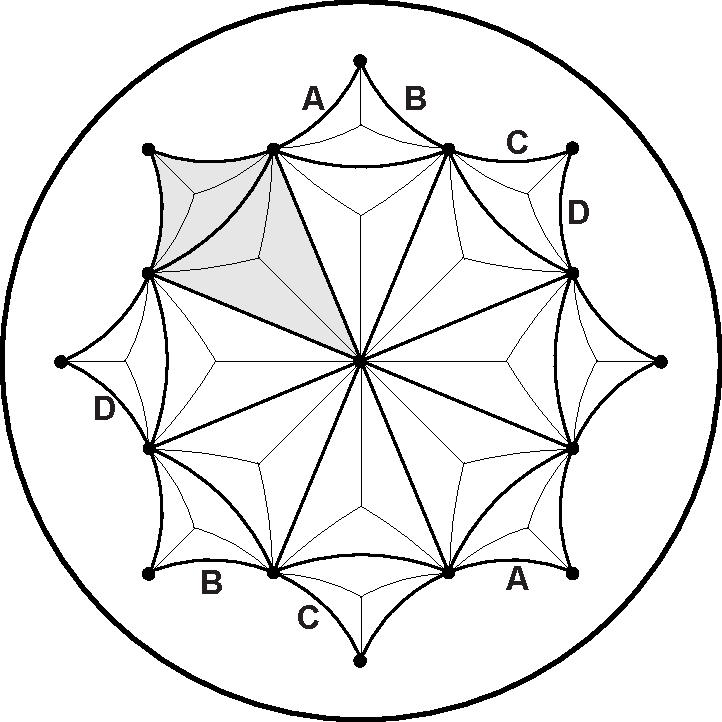
\includegraphics[width=2.75in]{figures/134_hyp}}}
    \qquad
    \subfloat[Flat 8-gon represents $\omega_1$ of $8(1 ,3, 4)$]{{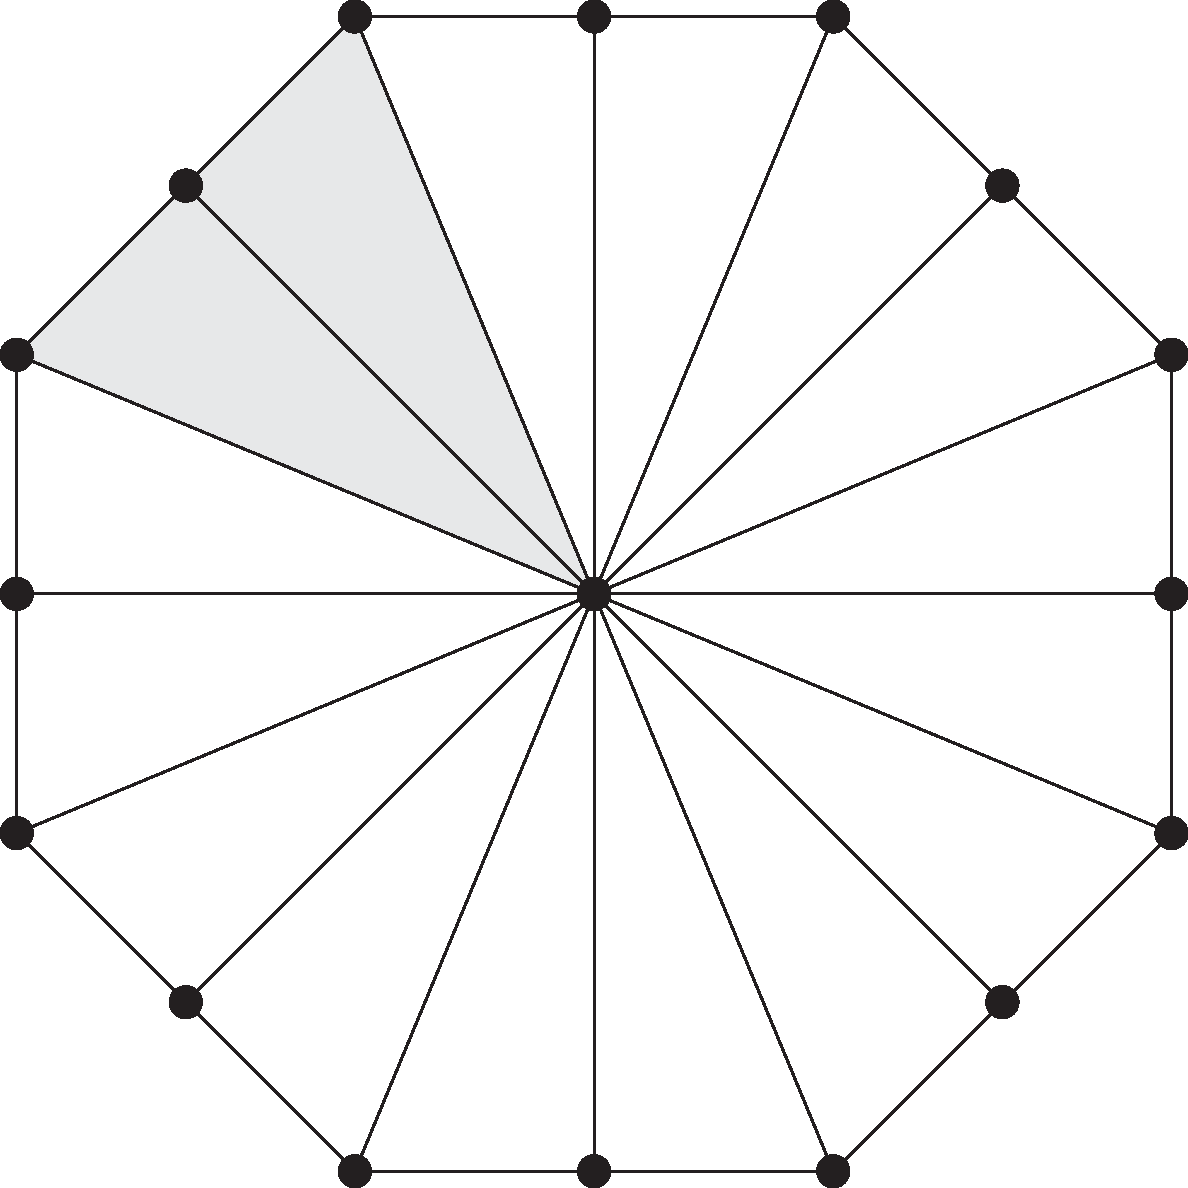
\includegraphics[width=2.75in]{figures/134_flat}}}%
    \caption{8(1, 3, 4)}%
    \label{fig:134}%
\end{figure}

In Figure~\crefformat{figure}{~#2#1{(b)}#3} \cref{fig:134}, we identify opposite edges and use the 1-forms achieved via multipliers. Then the period matrix is 

$$(\Pi) := (A | B) = \begin{pmatrix}1 & \frac{1 + i}{\sqrt{2}} & i & \frac{-1 + i}{\sqrt{2}}\\
1 & \frac{-1 + i}{\sqrt{2}} & -i & \frac{1 + i}{\sqrt{2}} \end{pmatrix}.$$


% In Figure~\crefformat{figure}{~#2#1{(a)}#3} \cref{fig:134}, the base tessellation yields we achieve a tessellation where all vertices are Weierstrass points. Moreover, all vertices on octahedron are similar. Hence, the group of automorphisms acts transitively on the tessellation. We have an order-sixteen rotation $a$ that fixes the center of the tessellation and an order-three rotation $b$ that fixes a triangle. Hence, $\Aut = \langle a, b | a^{16} = b^3 = 1 \rangle$ and $|\Aut| = 48.$ 

\subsection*{6(1, 1, 4)}

In this section, we look at another genus two curve defined by branching indices $6(1, 1, 4).$ It is a double cover over a doubled-hexagon and its plane curve model is $y^2 - (x^6 - 1).$ We cannot apply the base tessellation (Definition~\ref{defn: base tess}) here. Instead we tile the disc with twelve $(\frac{\pi}{3}, \frac{\pi}{6}, \frac{\pi}{6})$-triangles. These angles come from Gauss-Bonnet formula. Then we refine the tessellation so that the Weierstrass points are vertices of the tiling. Note that the center of Figure~\crefformat{figure}{~#2#1{(a)}#3} \cref{fig:114} is fixed under the sixfold map, not the hyperelliptic map. 

\begin{figure}[htbp]
    \centering
    \subfloat[Hyperbolic tessellation on $6(1, 1, 4)$]{{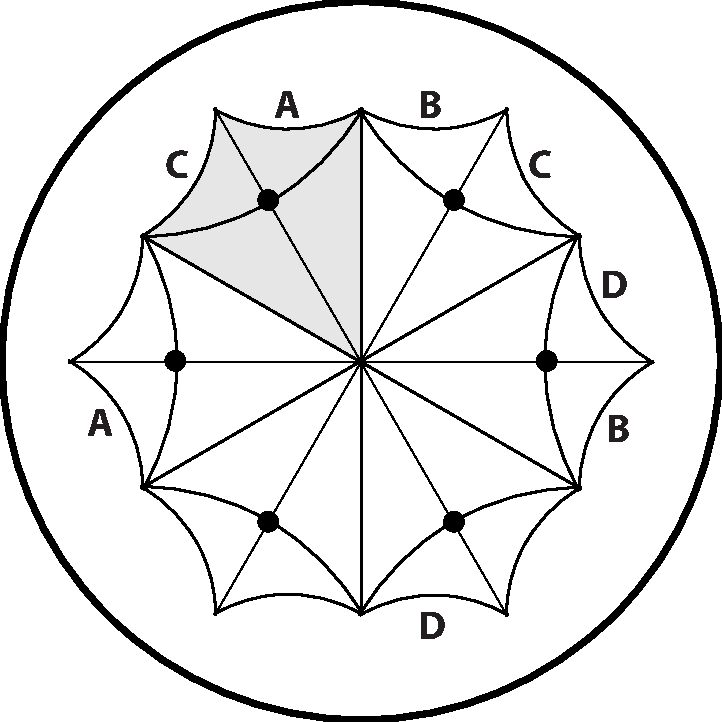
\includegraphics[width=2.75in]{figures/114_hyp}}}
    \qquad
    \subfloat[Flat 12-gon represents $\omega_1$ of $6(1, 1, 4)$]{{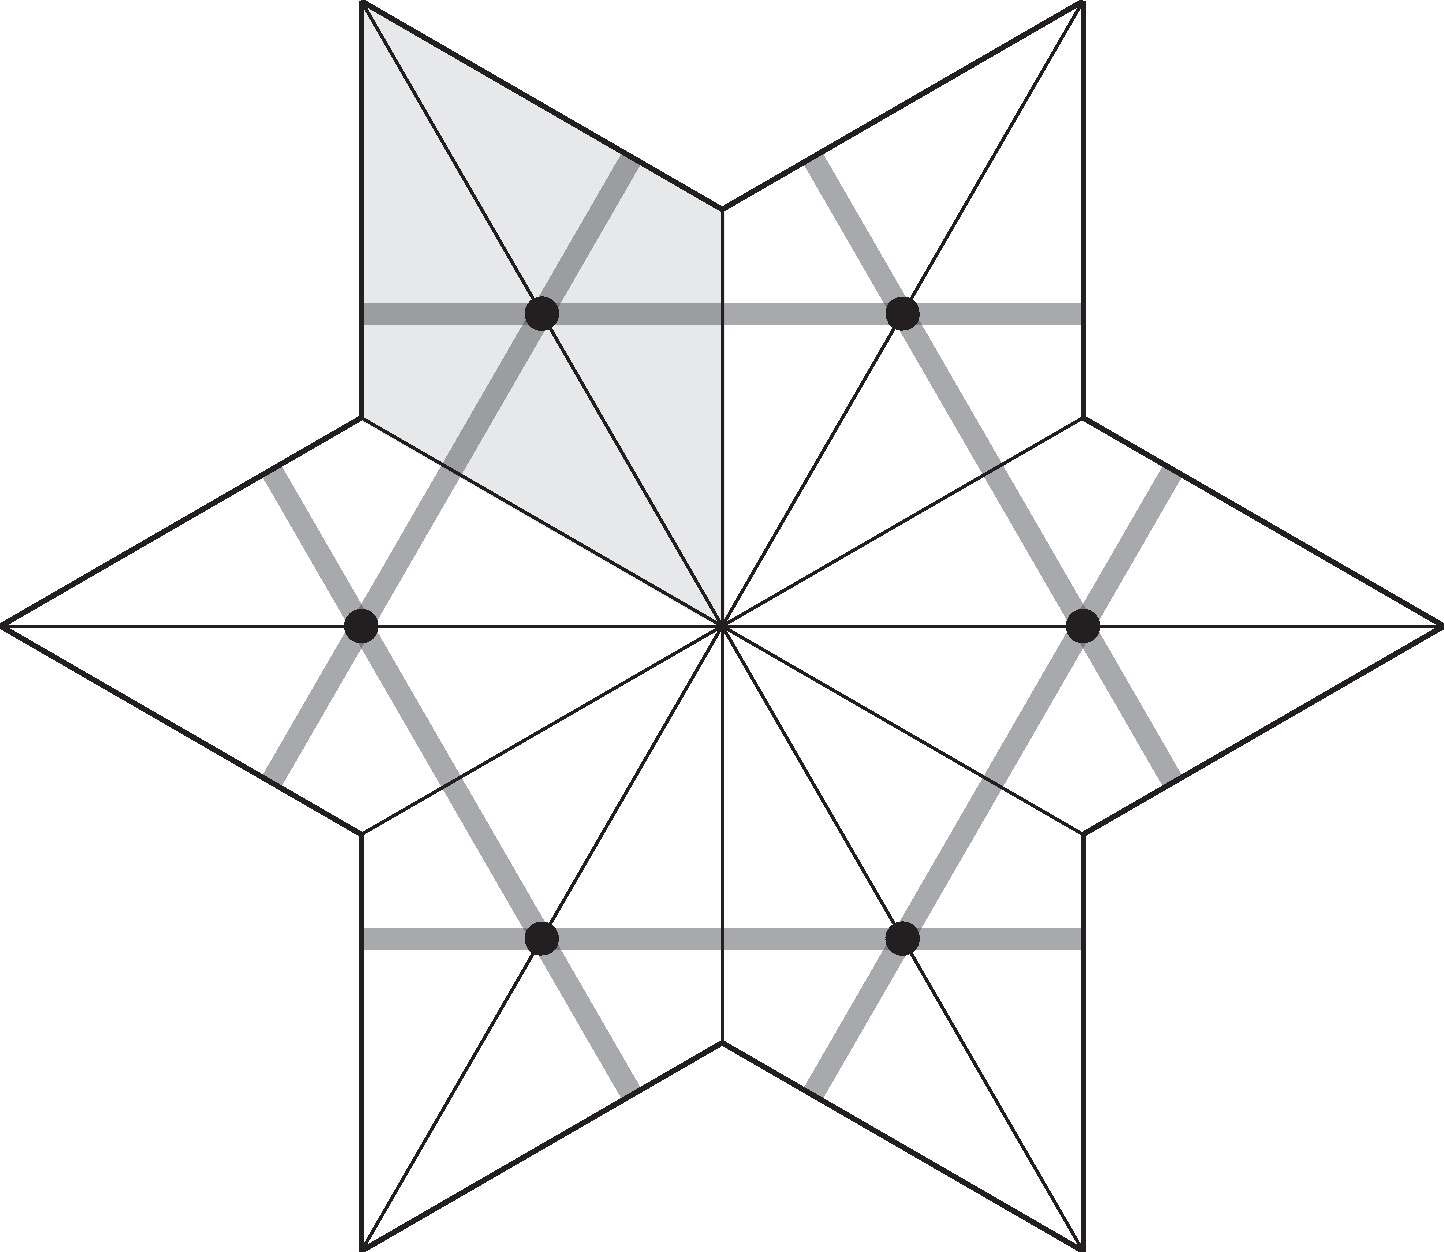
\includegraphics[width=2.75in]{figures/114_flat}}}%
    \caption{6(1, 1, 4)}%
    \label{fig:114}%
\end{figure}


The shaded area in Figure~\ref{fig:114} indicates a quotient sphere (under the sixfold map) and the Weierstrass points are denoted by $\bullet.$ The gray lines in Figure~\crefformat{figure}{~#2#1{(b)}#3} \cref{fig:114} indicate the identification of edges. We use the gray cycles as the homology basis and the 1-forms achieved via multipliers. Then the period matrix is

$$(\Pi) := (A | B) = \begin{pmatrix}1 & \frac{1 + \sqrt{3} i}{2} &  \frac{-1 + \sqrt{3} i}{2} & -1\\
1 & \frac{-1 + \sqrt{3} i}{2} & \frac{-1 - \sqrt{3} i}{2} & 1 \end{pmatrix}.$$

% In Figure~\crefformat{figure}{~#2#1{(a)}#3} \cref{fig:114}, we have a tessellation of the surface with similar triangles. All triangles have one vertex that is a Weierstrass point, and two vertices that are generic points. That is, not all vertices are similar. Since automorphisms preserve weights of points, given any two triangles in the tessellation, there exists only one map that maps one to the other. To compute $|\Aut|,$ we simply count the number of triangles in the tessellation.


%\subsection{7(1, 2, 4) Klein's quartic } 
%\begin{dami} do we say more about Klein here besides the things mentioned in chapter 3? if so, we can remove this subsection \end{dami}


%We refer the reader to Section ~\ref{sec:chap3} for details on Klein's quartic. 


%$x^3*y + y^3z + xz^3 $


%It is well known that $Aut(K) \simeq GL_3(F_2)$, and we reproved this by \texttt{autplane.sage}.

%G:= Group([[0,0,1,0,0,1],[1,-1,0,1,0,0],[0,0,0,1,1,0],[0,0,-1,0,0,0],[0,0,0,0,-1,0],[-1,0,0,-1,0,0]],[[0,0,1,0,1,1],[0,1,0,0,0,1],[0,0,0,1,0,0],[0,0,-1,0,-1,0],[0,0,0,0,1,0],[-1,0,0,-1,0,0]], [[0,0,1,0,0,1],[-1,1,0,-1,0,0],[-1,1,0,0,1,0],[-1,1,-1,-1,0,0],[1,0,1,0,0,1],[0,-1,0,0,0,0]], [[0,0,1,0,1,1],[0,-1,0,0,0,-1],[0,-1,0,1,0,-1],[0,-1,-1,0,-1,-1],[1,0,1,0,0,1],[-1,1,0,-1,0,1]], [[0,-1,0,-1,-1,0],[0,0,1,0,0,0],[0,0,0,1,0,0],[0,1,0,0,0,0],[0,0,0,-1,0,1],[-1,1,-1,-1,0,0]])

%535

\subsection*{8(1, 2, 5) Fermat's quartic}
%f4

This example arises in \cite{dami} as an abstract quotient of a triply periodic polyhedral surface. The polyhedral surface is called the Octa-4 as it is the boundary of a polyhedron built by gluing four regular octahedra to a centered octahedron. In \cite{dami}, the first author shows that the polyhedral metric induces hyperbolic structures and various translation structures that are compatible with its conformal type. It can also be written as an eightfold cyclic cover over a sphere defined by branching indices $(1, 2, 5).$ Via multipliers we achieve a basis of holomorphic 1-forms and find an explicit algebraic description of the surface that implies Fermat's quartic. 

% in case we want to include base tessellation use figures/125_base.pdf
% We begin with the base tessellation and proceed as we do in the case of Klein's quartic. 

\begin{figure}[htbp]
    \centering
    \subfloat[Hyperbolic tessellation on $8(1, 2, 5)$]{{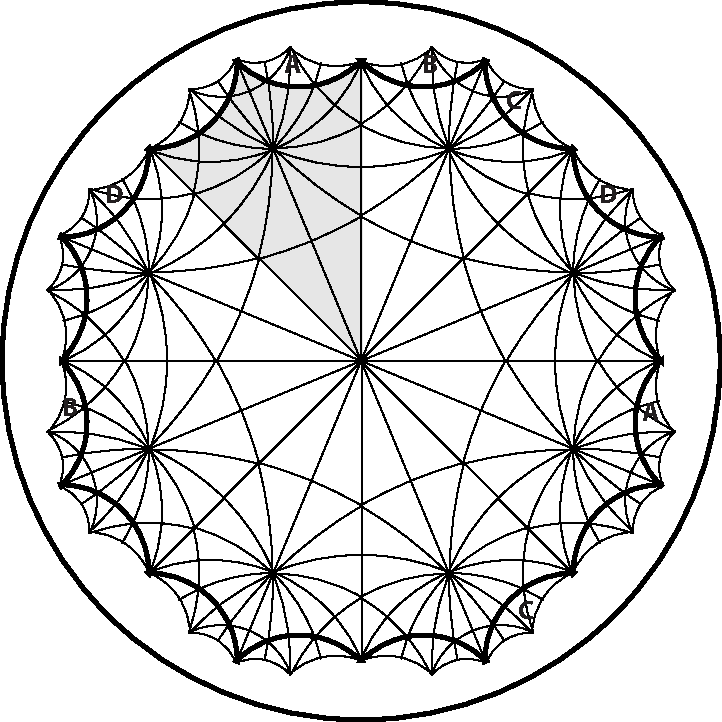
\includegraphics[width=2.75in]{figures/125_hyp}}}
    \qquad
    \subfloat[Flat sixteengon represents $\omega_1$]{{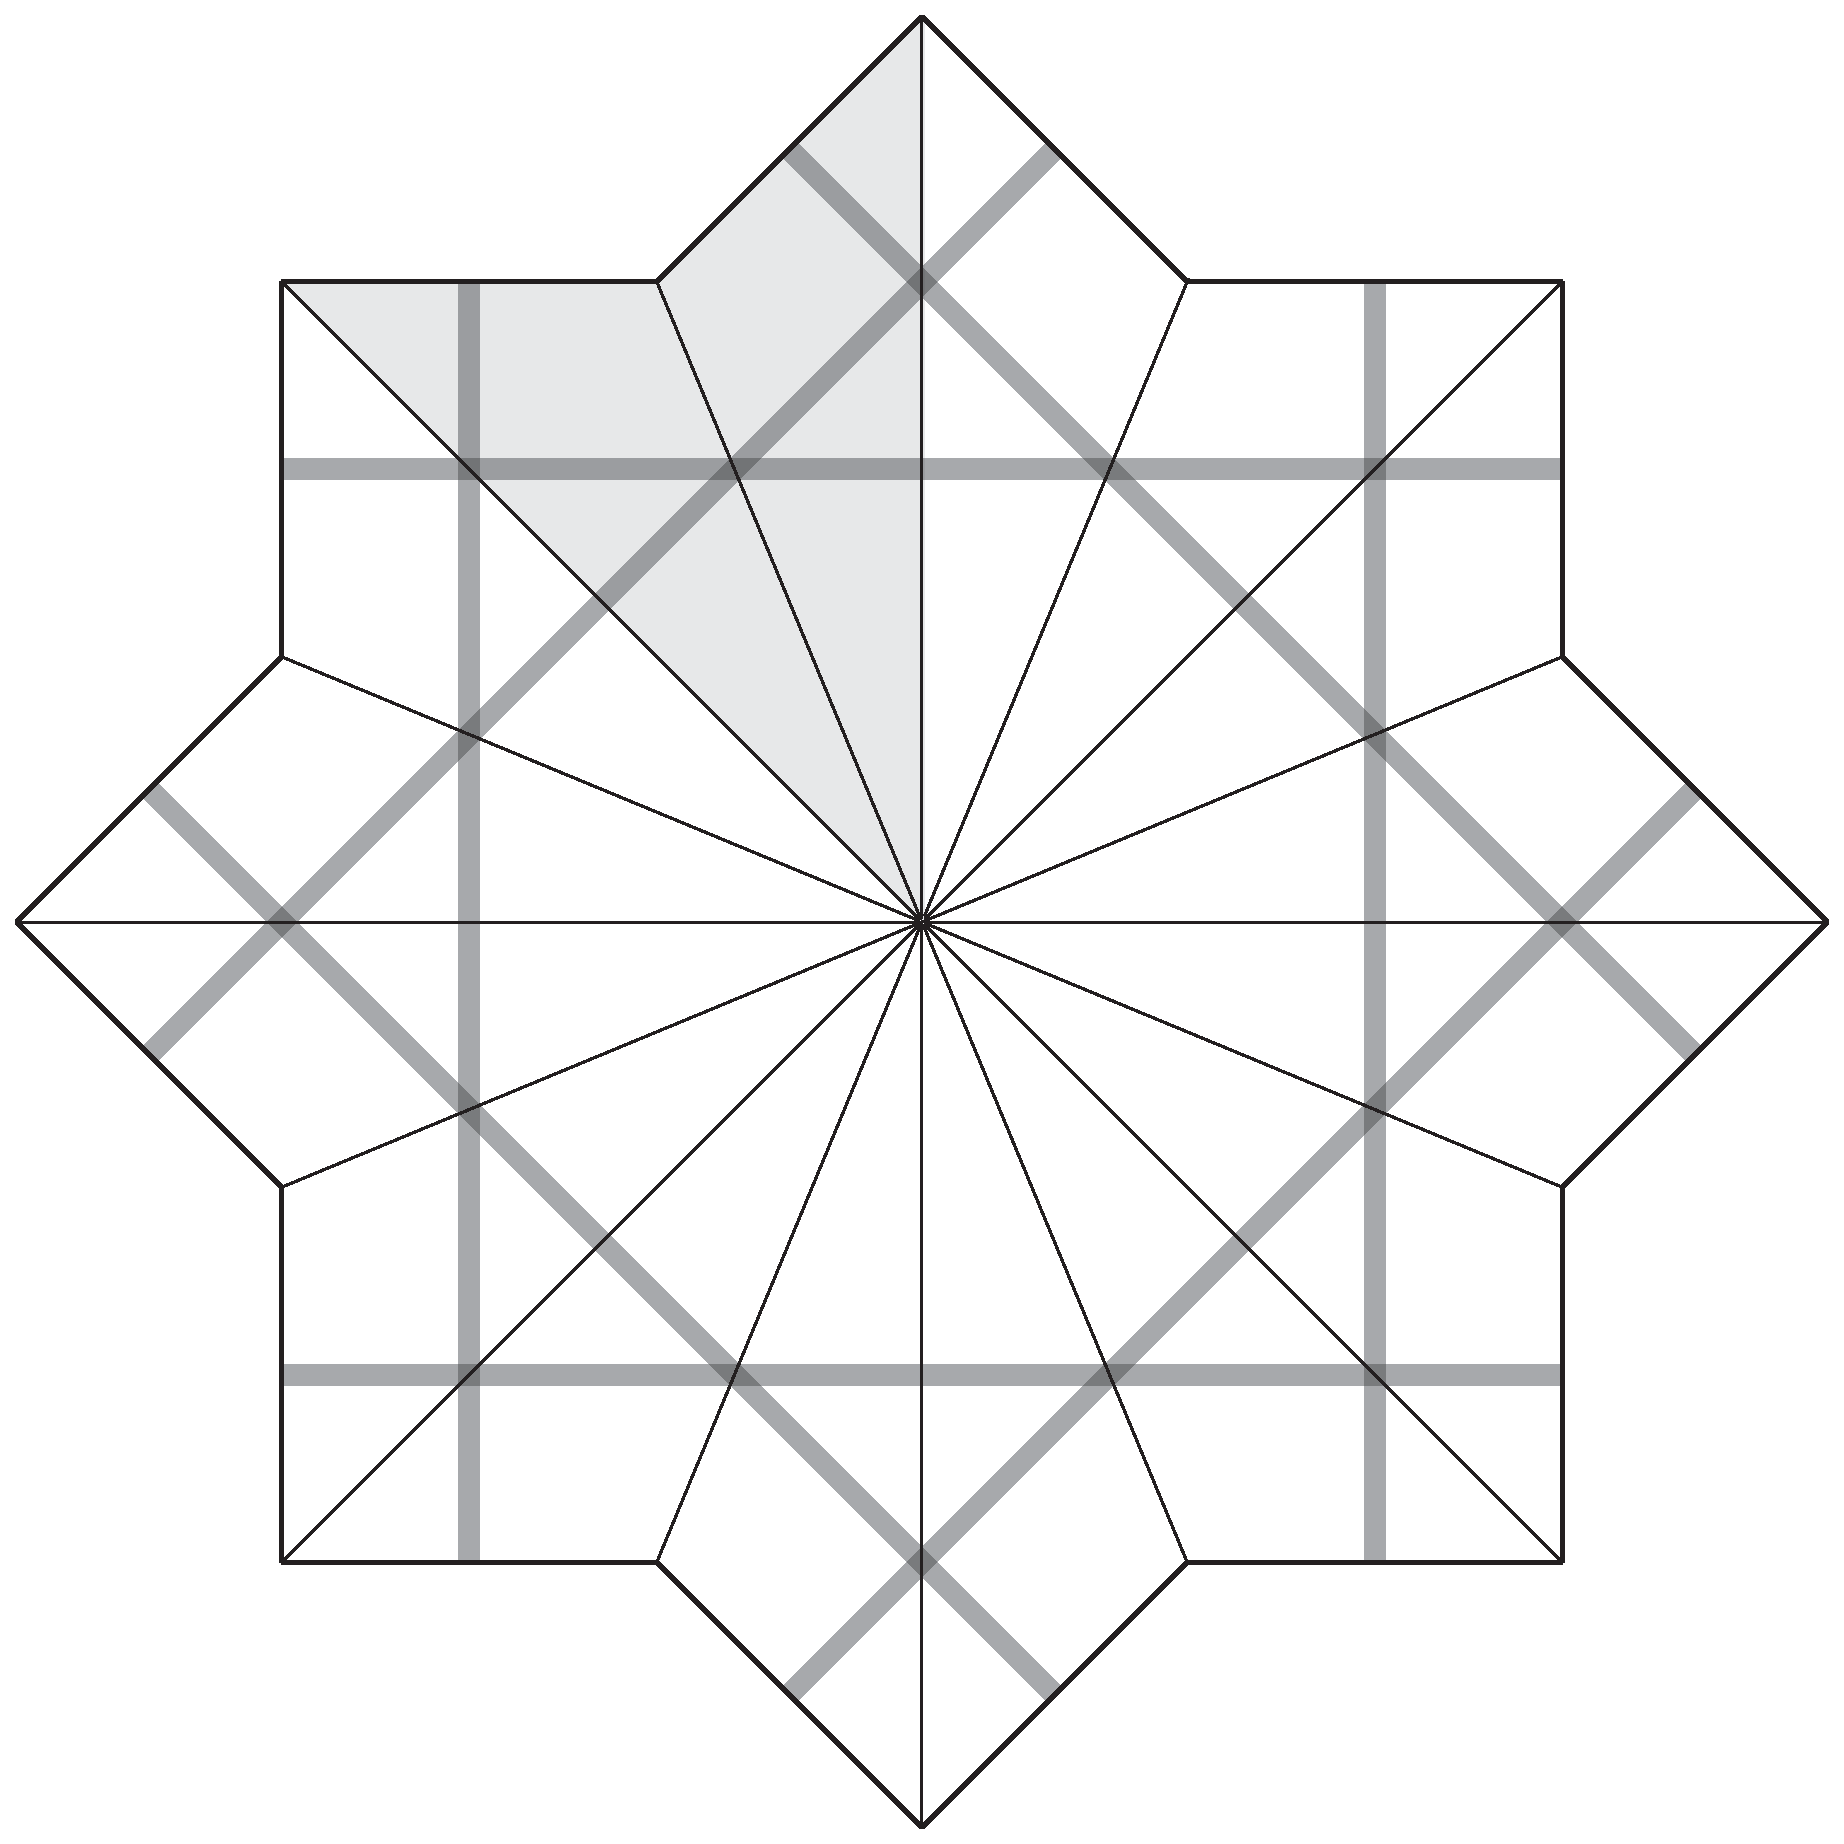
\includegraphics[width=2.75in]{figures/125_flat}}}%
    \caption{8(1, 2, 5)}%
    \label{fig:125}%
\end{figure}

In \cite{dami}, the author shows that the eightfold cover defined over $\mathbb{S}^2 \setminus \{p_1, p_2, p_3\}$ can also be written as a fourfold cyclic cover over $\mathbb{S}^2 \setminus \{q_1, q_2, q_2', q_3\}$ defined by 4(1, 1, 1, 1). We identify $p_i$ and $q_i$ such that $p_i = q_1$ for $i = 1$ and $i = 3,$ and $\widetilde{p_2} = \widetilde{q_2}$ and $\widetilde{p_2}_2 = \widetilde{q_2'}.$ Then the two affine models $y^8 - x(x - 1)^5$ are equivalent $y^4 - x (x - 1) (x + 1),$ and given the latter we achieve Fermat's quartic.

%We can reuse the hyperelliptic dummy, as our genus is still 3.

%\begin{theorem} \cite{dami} $Octa\text{-}4$ is nonhyperelliptic and of genus 3. $Aut(Octa\text{-}4) \simeq (C_4)^2 \rtimes S_3$. This is is a group of order 96. \end{theorem}

%\begin{proof} Alternative proof: by \texttt{autplane.sage}. \end{proof}

\begin{remark} It was presented in the paper \cite{dami} as $\Aut(X) = \langle a, b \mid a^8 = b^3 = (ab) ^2 = (a^2b^2)^3 = (a^4b^2)^3 = 1 \rangle$, but this is equivalent to the group in Table ~\ref{table:pp} by the GAP small group identification function. We reproved this with \texttt{autplane.sage}. \end{remark}

%710 PP

Using the same method as earlier, that is, so that the intersection matrix is chosen as

$$\textrm{int}_1 = \begin{pmatrix} 0 & 1 & 1 & 0 & 0 & 0 \\
 -1 & 0 & 1 & 1 & 0 & 0 \\
 -1 & -1 & 0 & 1 & 1 & 0 \\
 0 & -1 & -1 & 0 & 1 & 1 \\
 0 & 0 & -1 & -1 & 0 & 1 \\
 0 & 0 & 0 & -1 & -1 & 0 \end{pmatrix},$$

the period matrix $\Pi_1$ is computed as follows: 
$$\P_1 = \left(
\begin{array}{cccccc}
 1 & e^{\frac{\pi i}{4}} & i & e^{\frac{3 \pi i}{4}} & -1 & e^{-\frac{3 \pi i}{4}} \\
 1 & i & -1 & -i & 1 & i \\
 1 & e^{-\frac{3 \pi i}{4}} & i & e^{-\frac{\pi i}{4}} & -1 & e^{\frac{\pi i}{4}} 

\end{array}
\right)$$
 
\begin{remark} In \cite{dthesis}, the homology basis is chosen so that the cycles appear as ``handles'' on the polyhedral surface. That is, 
$$\textrm{int}_2 = \begin{pmatrix} 0 & 0 & 0 & 1 & 0 & 0 \\
 0 & 0 & 0 & 0 & 1 & 0 \\
 0 & 0 & 0 & 0 & 0 & 1 \\
 -1 & 0 & 0 & 0 & 0 & 0 \\
 0 & -1 & 0 & 0 & 0 & 0 \\
 0 & 0 & -1 & 0 & 0 & 0\end{pmatrix}$$


This yields the following period matrix $\Pi_2$ 
$$\Pi_2 = (A|B) = \begin{pmatrix}  1 - i& -((1 + i)/(1 + \sqrt{2}))& (1 + i)/(1 + \sqrt{2})& 1 + i& \sqrt{2}& 2 - \sqrt{2} \\  -2i& 2i& 2i& 2i& -2& -2\\ -1 - i & (1 - i)(1 + \sqrt{2})& (-1 + i)(1 + \sqrt{2})& 1 - i& i\sqrt{2}& i(-2 - \sqrt{2})  \end{pmatrix} $$ and $$\tau = (A^{-1}B) = \begin{pmatrix}i & \frac{1 + i}{2} & \frac{1 + i}{2}\\
\frac{1 + i}{2} & i & \frac{1 + i}{2}\\
\frac{1 + i}{2} & \frac{1 + i}{2} & i\end{pmatrix}$$
\end{remark}


\subsection*{12(1, 3, 8)}

%f8 
In this section, we look at an example that arises from the Shiga curve $y^3 = x^4 - 1.$ We observe that there is an order-twelve map $x \mapsto i x,$ $y \mapsto \zeta y,$ where $\zeta$ is a third root of unity. As we have three branched values 0, 1, and $\infty,$ we look at twelvefold cyclic covers that are branched over a thrice punctured sphere. Appendix A of \cite{dthesis} tells us that there are two such covers. One is defined as $12(1, 5, 6)$ and the other is defined as $12(1, 3, 8).$ The former is hyperelliptic whereas the latter is not. Therefore we conclude that the Shiga curve corresponds to the $12(1, 3, 8)$ cover. 

The admissible cone metrics arise from multipliers and yield a basis of 1-forms with divisors $(\omega_1) = \widetilde{p_3}_1 + \widetilde{p_3}_2 + \widetilde{p_3}_3 + \widetilde{p_3}_4,$ $(\omega_2) = \widetilde{p_1} + \widetilde{p_2}_1 + \widetilde{p_2}_2 + \widetilde{p_2}_3,$ and $(\omega_3) = 4 \widetilde{p_1}.$ The Wronskian computation tells us that the Weierstrass points do not have equal weight: $\widetilde{p_1}$ and $\widetilde{p_2}_i$ have weight two, $\widetilde{p_3}_i$ have weight one. Additionally we have $\textrm{wt}(\widetilde{p_*}_i) = 1,$ where $p_*$ is the midpoint of $\overline{p_1 p_2}.$ To find a tessellation that is preserved under its automorphism group, we begin with the base tessellation. Gauss-Bonnet formula tells us that we must have sixteen hyperbolic $(\frac{\pi}{6}, \frac{\pi}{6}, \frac{\pi}{6})$-triangles. The region bounded by the bold lines shows the tessellation of the surface $12(1, 3, 8)$ in Figure~\crefformat{figure}{~#2#1{(a)}#3} \cref{fig:138}. We mark the Weiertrass points and subdivide the $(\frac{\pi}{6}, \frac{\pi}{6}, \frac{\pi}{6})$-triangles so that all triangles are congruent to each other. Vertices marked as $\bullet$ are Weierstrass points of weight two, those marked as $\circ$ are points of weight one. 

\begin{figure}[htbp]
    \centering
    \subfloat[Hyperbolic tessellation on $12(1, 3, 8)$]{{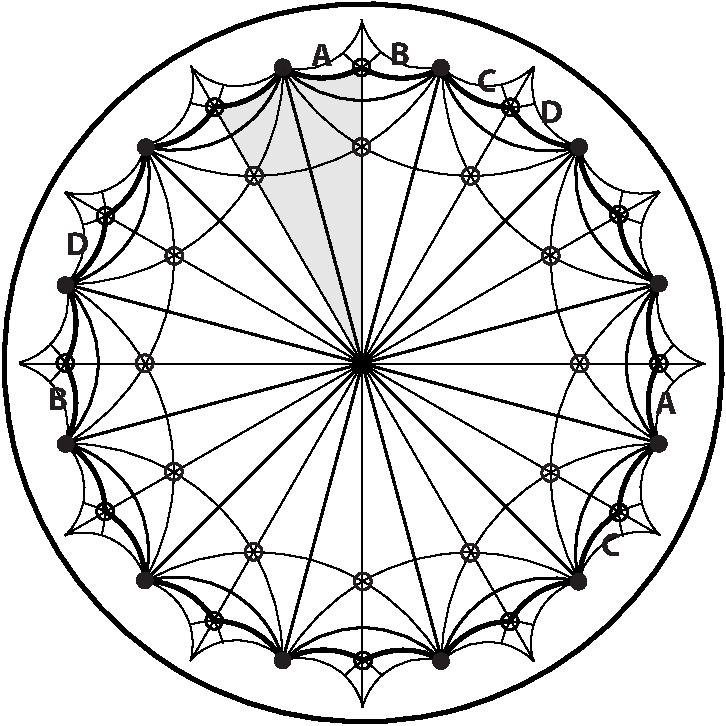
\includegraphics[width=2.75in]{figures/138_hyp}}}
    \qquad
    \subfloat[Flat 24-gon represents $\omega_1$ of $12(1, 3, 8)$]{{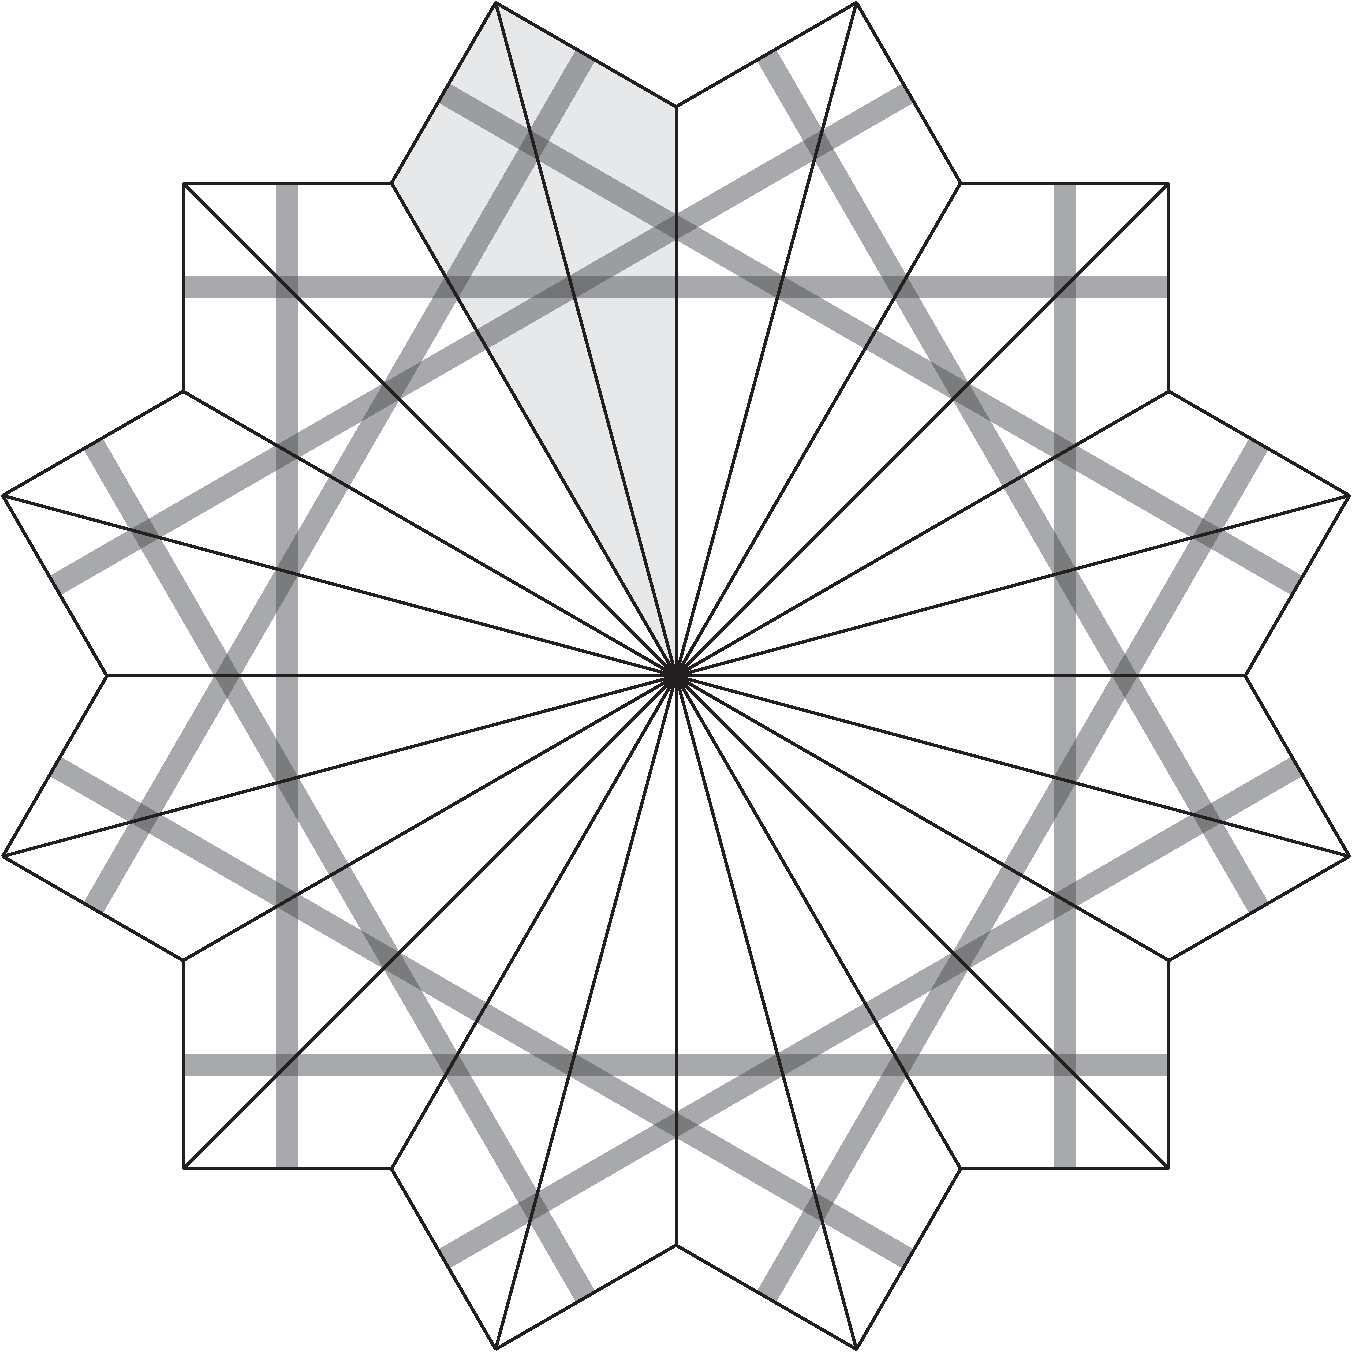
\includegraphics[width=2.75in]{figures/138_flat}}}%
    \caption{12(1, 3, 8)}%
    \label{fig:138}%
\end{figure}


% Let $a$ be an order-twelve rotation that fixes the center of the tessellation, and $b$ be an involution that fixes an edge that connects two points marked as $\circ.$ Since automorphisms preserve weights of points, given any two triangles in the tessellation, there exists only one map that maps one to the other. 

%\begin{theorem} $Aut(X8)\simeq \times (C_4 \cdot A_4)$.  The order of this group is 48. \end{theorem}

%\begin{remark} Here, $C_4 \cdot A_4$ denotes the central extension by $C_4$ of $A_4$ (i.e., SmallGroup(48, 33)). \end{remark}
The period matrix of $12(1, 3, 8)$ is: 

$$\Pi = \begin{pmatrix} 1 & e^{\frac{\pi i}{6}} & e^{\frac{\pi i}{3}} & i & e^{\frac{2 \pi i}{3}} & e^{\frac{5 \pi i}{6}} \\
 1 & e^{\frac{\pi i}{3}} & e^{\frac{2 \pi i}{3}} & -1 & e^{-\frac{2 \pi i}{3}} & e^{-\frac{\pi i}{3}} \\
 1 & e^{\frac{5 \pi i}{6}} & e^{-\frac{\pi i}{3}} & i & e^{-\frac{2 \pi i}{3}} & e^{\frac{\pi i}{6}} \\
\end{pmatrix}$$

 %The program \texttt{autperio.sage} found only 1 principal polarization up to automorphism-equivalence. Of course $Aut(J(X8, a)) \simeq  (C_4 \cdot A_4) \times C_2$ (of order 96) with respect to this principal polarization $a$. 

\subsection*{8(1, 1, 6)}
In this section, we look at a genus three hyperelliptic curve. We find its base tessellation with thirty two 8-valent triangles. Via the Wronskian we locate the Weierstrass points and refine the tessellation to show all symmetries (Figure~\crefformat{figure}{~#2#1{(a)}#3} \cref{fig:116}). These points are fixed under the hyperelliptic involution, whose quotient is a doubled-octagon, hence the plane curve model is $y^2 - (x^8 - 1).$ 

\begin{figure}[htbp]
    \centering
    \subfloat[Hyperbolic tessellation on $8(1, 1, 6)$]{{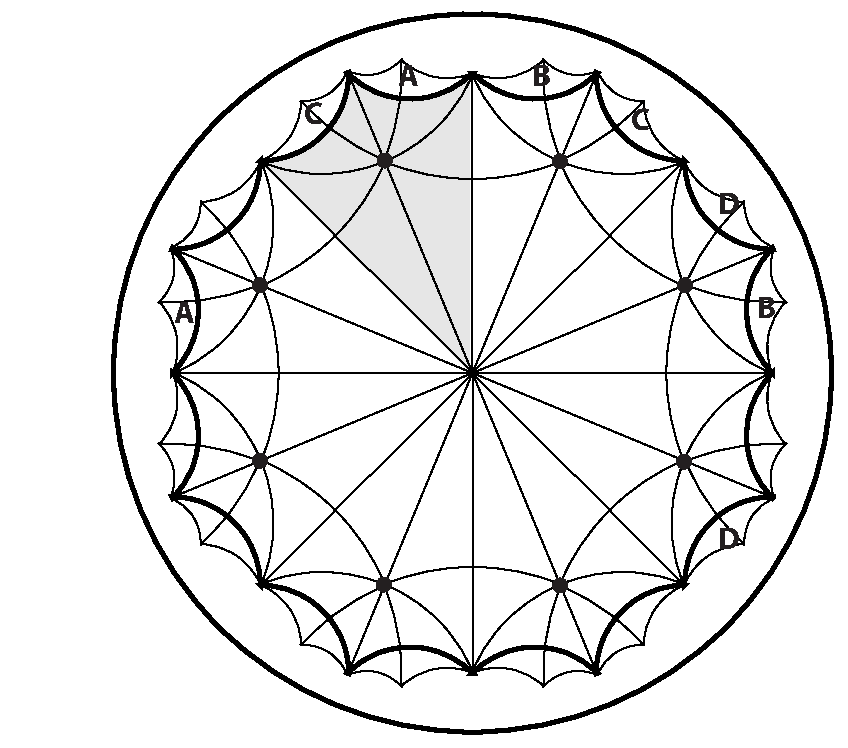
\includegraphics[width=2.75in]{figures/116_hyp}}}
    \qquad
    \subfloat[Flat 16-gon represents $\omega_1$ of $8(1, 1, 6)$]{{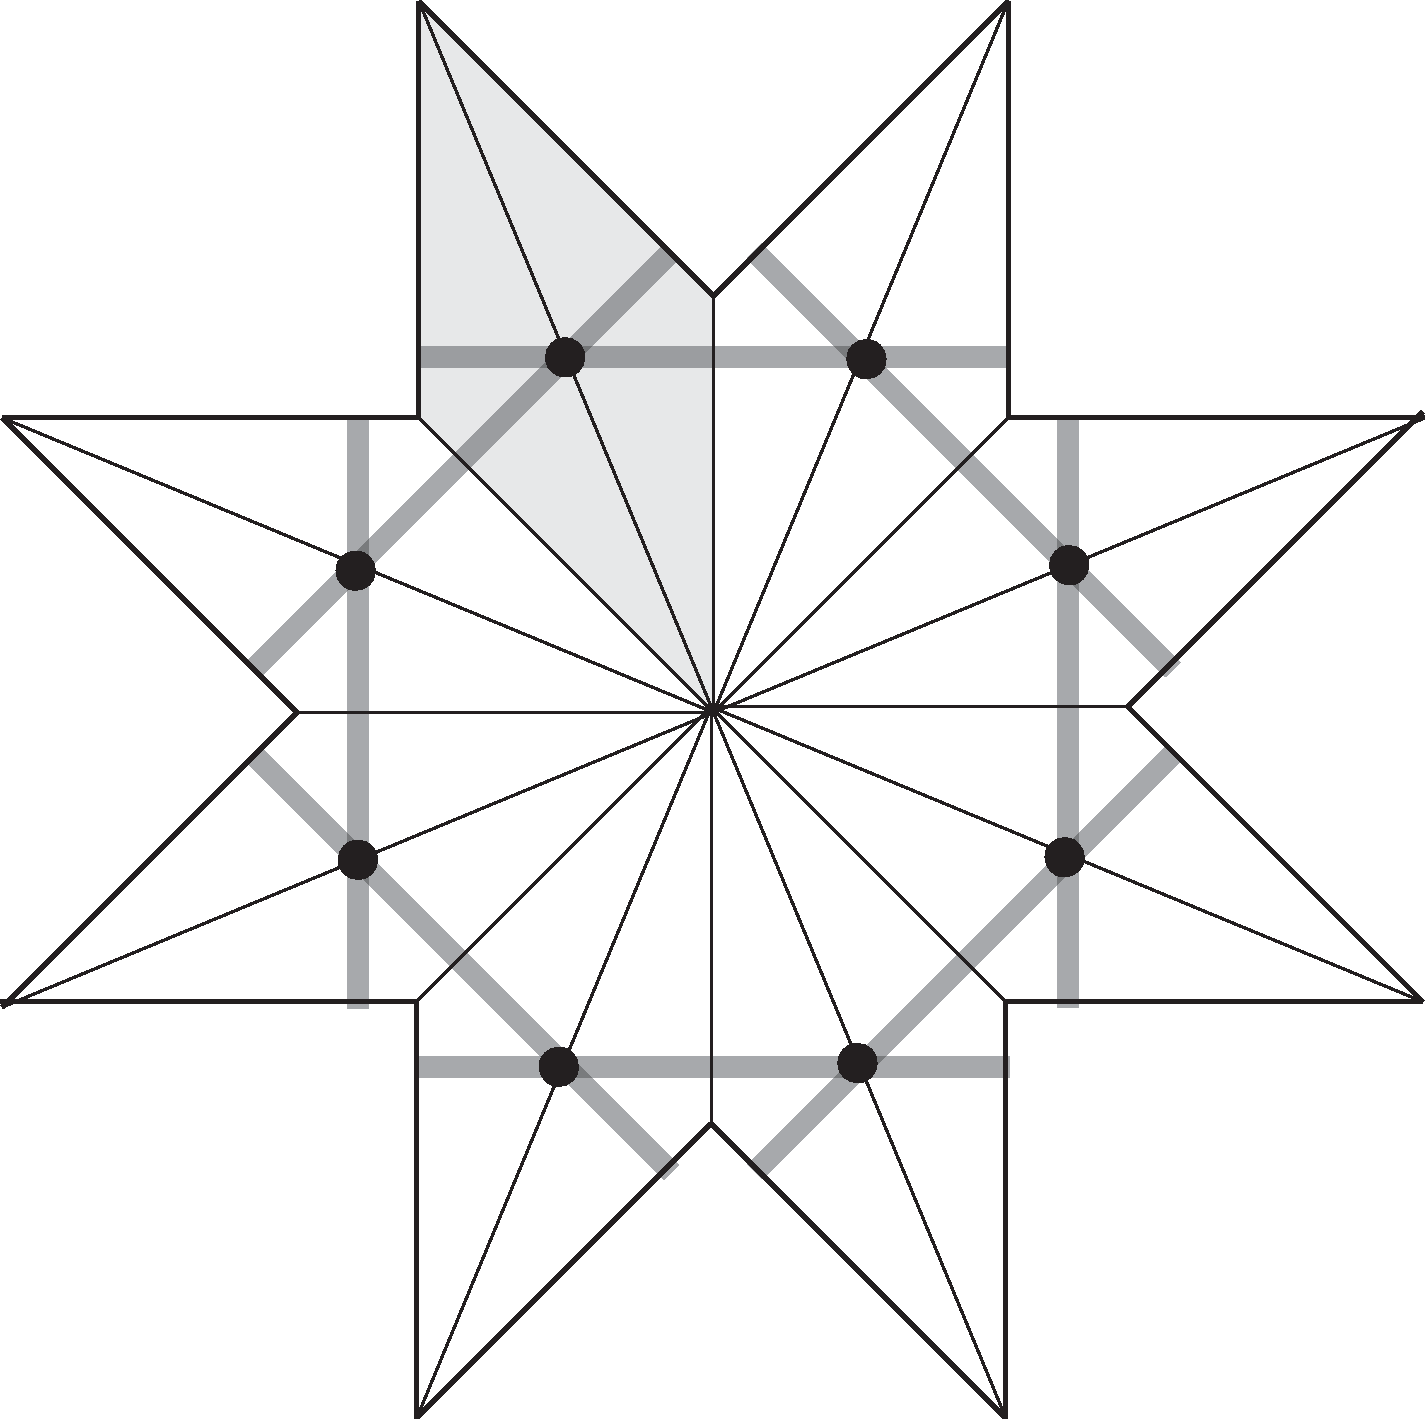
\includegraphics[width=2.75in]{figures/116_flat}}}%
    \caption{8(1, 1, 6)}%
    \label{fig:116}%
\end{figure}

The period matrix is 
$$\Pi := \begin{pmatrix}
 1 & e^{\frac{\pi i}{4}} & i & e^{\frac{3 \pi i}{4}} & -1 & e^{-\frac{3 \pi i}{4}} \\
 1 & i & -1 & -i & 1 & i \\
 1 & e^{\frac{3 \pi i}{4}} & -i & e^{\frac{\pi i}{4}} & -1 & e^{-\frac{\pi i}{4}} \end{pmatrix}.$$ 
 
% Similar to $6(1, 1, 4),$ the triangles on the tessellation are similar to each other, each with two vertices that are generic, and one vertex that is a Weierstrass point. Therefore, $|\Aut|$ corresponds to the number of triangles on the tessellation.


\subsection*{12(1, 5, 6)}
%f10

In this section, we look at another example of a genus three hyperelliptic surface which is defined by branching indices $12(1, 5, 6).$ It is a double-cover over a sphere with six branched points that are located at the North and South Pole, and six equidistributed points on the Equator. Hence, the plane curve model for this is $y^2 - x (x^6 - 1).$ Via Gauss-Bonnet formula, the base tessellation is tiled by twenty four hyperbolic $(\frac{\pi}{6}, \frac{\pi}{4}, \frac{\pi}{4})$-triangles. All Weierstrass points are marked as either $\bullet$ or $\circ$ as they have different valency.

\begin{figure}[htbp]
    \centering
    \subfloat[Hyperbolic tessellation on $12(1, 5, 6)$]{{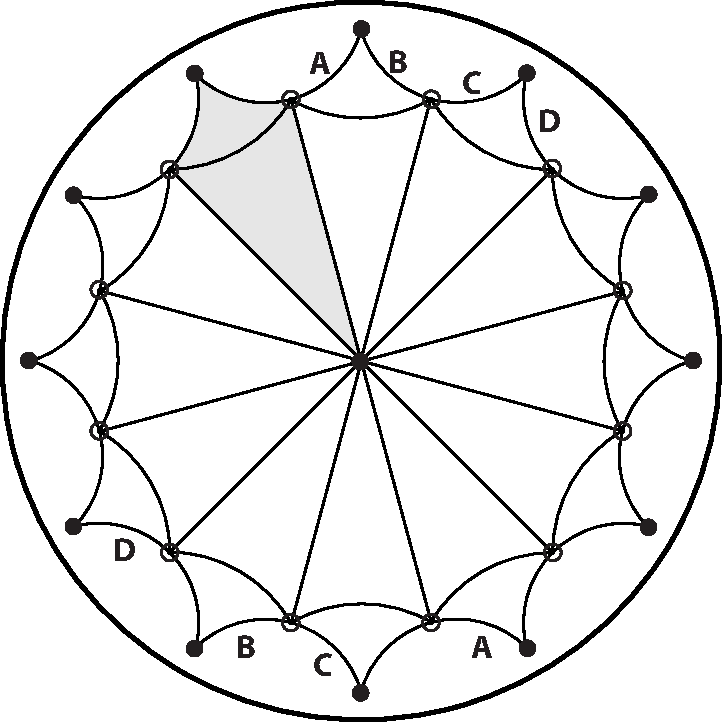
\includegraphics[width=2.75in]{figures/156_hyp}}}
    \qquad
    \subfloat[Flat 12-gon represents $\omega_1$ of $12(1, 5, 6)$]{{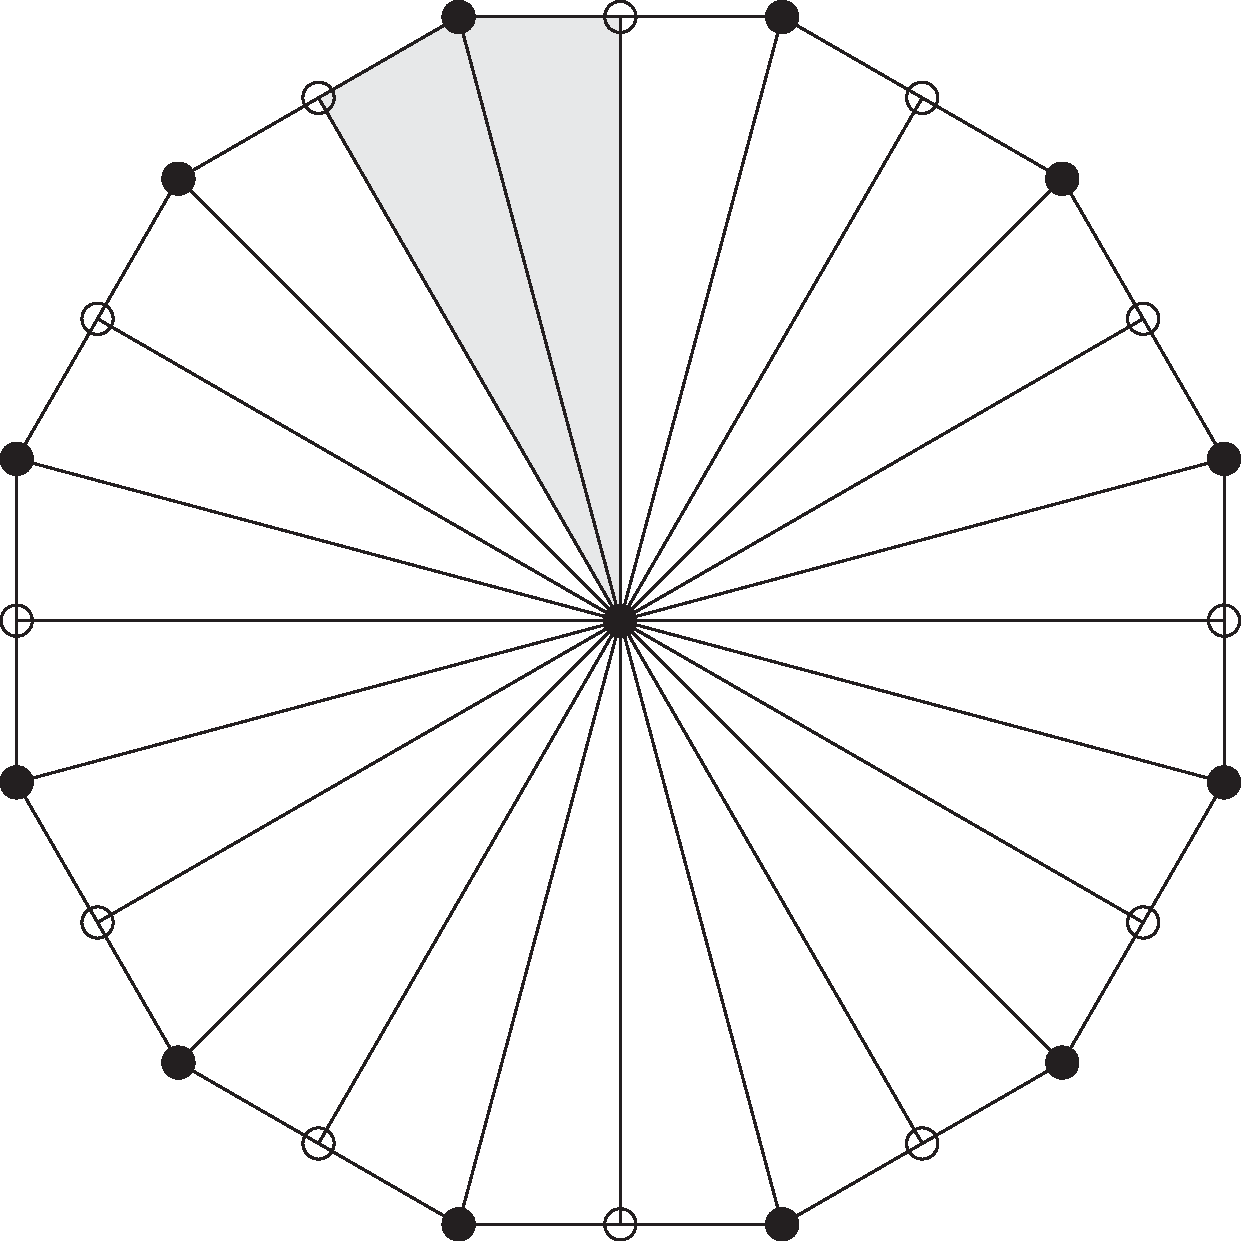
\includegraphics[width=2.75in]{figures/156_flat}}}%
    \caption{12(1, 5, 6)}%
    \label{fig:156}%
\end{figure}

%$X_{(156)}$ is a twelvefold cover with branching indices $12(1, 5, 6)$,

%\begin{lemma} X10 is hyperelliptic and of genus three. \end{lemma}


%It is infact https://groupprops.subwiki.org/wiki/Nontrivial_semidirect_product_of_Z3_and_Z8 

%\begin{remark} In particular, $Aut(J, a)$ is a semidirect product $C_2 \rtimes C_{12}$ ($C_2$ is normal), and the action $C_2 \to Aut(C_{12})$ sends $g \mapsto gmg^{-1} = m^5$. It is not obviously the usual dihedral or dicyclic group.\end{remark}

We use the identification of opposite edges of the 12-gon as the homology basis and the 1-forms achieved via multipliers. Then the period matrix of $12(1, 5, 6)$ is

$$\Pi = \begin{pmatrix}1 & e^{\frac{\pi i}{6}} & e^{\frac{2 \pi i}{6}} & e^{\frac{3 \pi i}{6}} & e^{\frac{4 \pi i}{6}} & e^{\frac{5 \pi i}{6}}\\
1 & e^{\frac{\pi i}{2}} & e^{\frac{2 \pi i}{2}} & e^{\frac{3 \pi i}{2}} & e^{\frac{4 \pi i}{2}} & e^{\frac{5 \pi i}{2}}\\
1 & e^{\frac{5 \pi i}{6}} & e^{\frac{10 \pi i}{6}} & e^{\frac{15 \pi i}{6}} & e^{\frac{20 \pi i}{6}} & e^{\frac{25 \pi i}{6}}\end{pmatrix}$$

% On its tessellation (Figure~\crefformat{figure}{~#2#1{(a)}#3} \cref{fig:156}), all vertices are Weiertrass points of equal weight. However, by identification of edges, one can see that not all vertices are similar. At the center of the tessellation is 12-valent but not all vertices are. Hence, we denote them with different markings. Then by the same argument as in $6(1, 1, 4),$ $12(1, 3, 8),$ and $8(1, 1, 6),$ $|\Aut|$ equals the number of triangles that appear on the tessellation.

\subsection*{4(1, 3, 3, 1)}

 %f9
In this section, we look at a cyclic cover that is branched over a 4-punctured sphere. In our case, the admissible cone metrics are achieved via multipliers, although this is not true for all cyclically branched covers over $n (\geq 4)$-punctured spheres (See chapter~\ref{sec:chap3}). We begin with a base tessellation by eight $(\frac{\pi}{4}, \frac{\pi}{4}, \frac{\pi}{4}, \frac{\pi}{4})$-squares. The admissible cone metrics yield a basis with divisors $(\omega_1) = 2 \widetilde{p_2} + 2 \widetilde{p_3},$ $(\omega_2) = \widetilde{p_1} + \widetilde{p_2} + \widetilde{p_3} + \widetilde{p_4},$ and $(\omega_3) = 2 \widetilde{p_1} + 2 \widetilde{p_4}.$ Given a chart where $(z(p_i)) = (-a, -1, 1, a)$ for some $a > 1,$ the Wronskian tells us that the curve is hyperelliptic and the Weierstrass points are located at the preimages of $q$ where $z(q) = 0$ or $z(q) = \infty.$ The Weierstrass points are marked as $\bullet$ in Figure~\crefformat{figure}{~#2#1{(a)}#3} \cref{fig:1331}.

% explain how h.e. involution works wrt a and b?
 
\begin{figure}[htbp]
    \centering
    \subfloat[Hyperbolic tessellation on 4(1, 3, 3, 1)]{{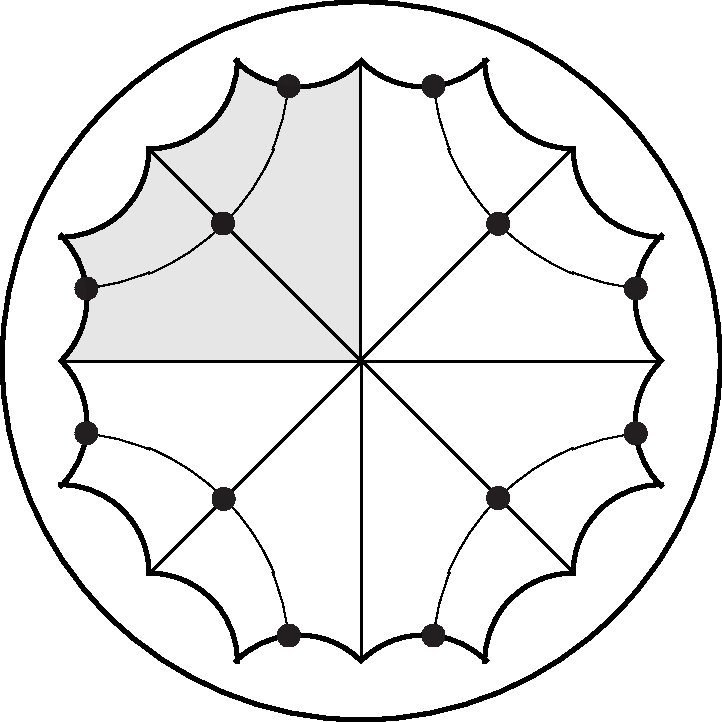
\includegraphics[width=2.75in]{figures/1331_flag}}}%
    \qquad
    \subfloat[flat, $a = \sqrt{2}$]{{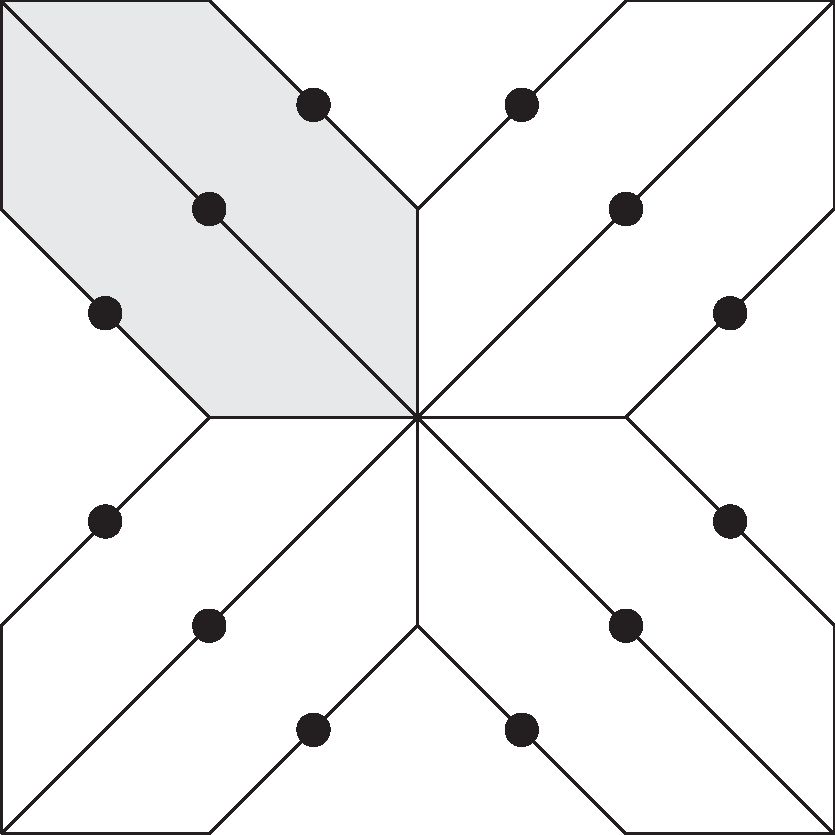
\includegraphics[width=2in]{figures/1331_flat}}}
   \qquad
    \subfloat[flat, $a = \sqrt{5}$]{{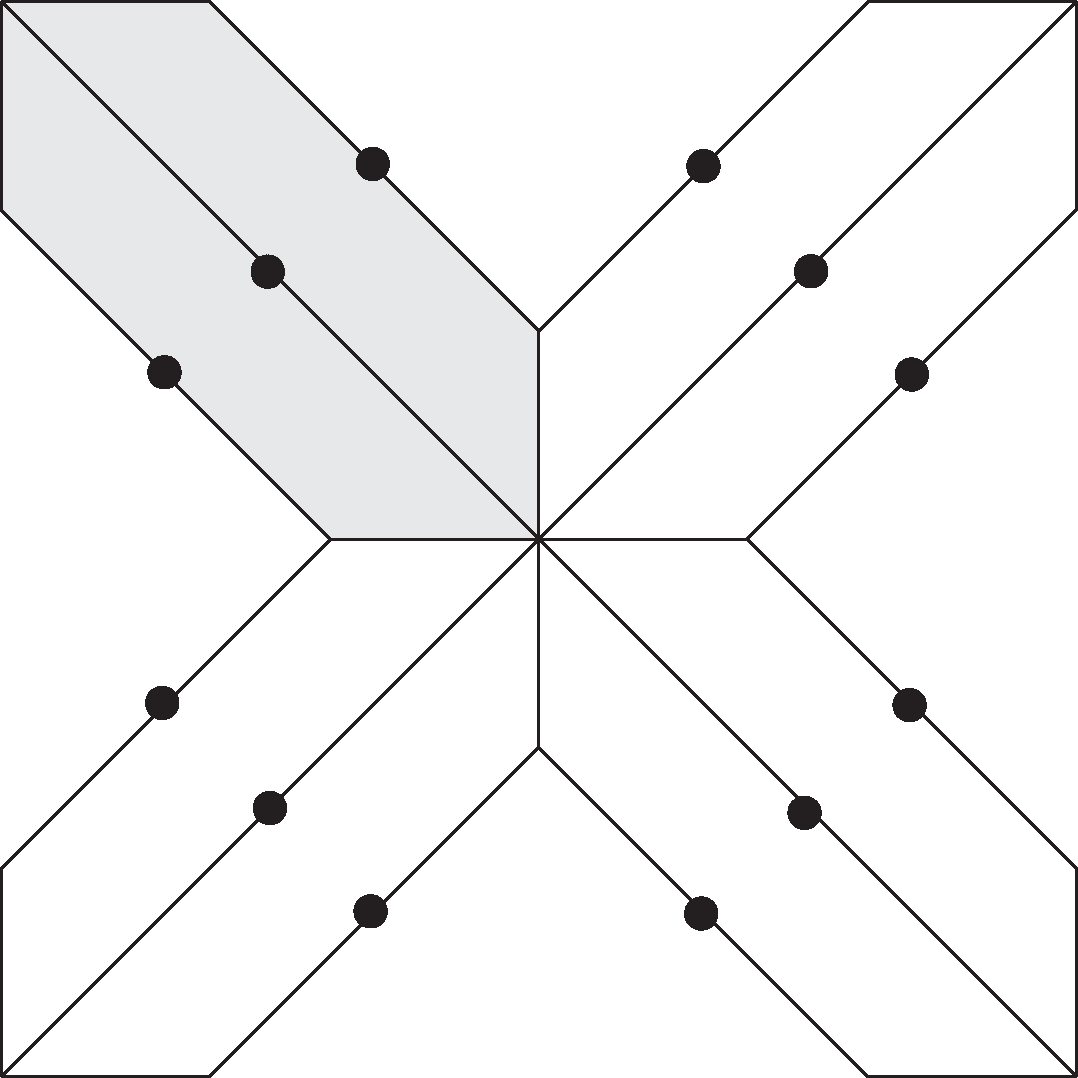
\includegraphics[width=2in]{figures/1331_flat_sqrt5}}}%
    \caption{4(1, 3, 3, 1)}%
    \label{fig:1331}%
\end{figure}

Given the branching indices, that is, the appropriate cone angles, the four punctured sphere associated to $\omega_1$ is a doubled trapezoid with angles $\frac{\pi}{4}$ and $\frac{3 \pi}{4}.$ However, the trapezoid cannot be pinned down uniquely (Figure~\ref{fig:1331}). However, we set the side lengths of the trapezoid so that $\overline{p_1 p_2} = 1$ and $\overline{p_2 p_3} = b$ for $b > 0.$ For $\omega_2,$ the cone angles are $\frac{\pi}{2}$ at each puncture. We take the side lengths to be 1 and $c,$ and show that $c$ can be arbitrary. Given $b, c >0,$ we calculate the period matrix to be:

$$\Pi = \begin{pmatrix} 1 & i & -1 & (b + \sqrt{2}) e^{\frac{i \pi }{4}} & (b + \sqrt{2}) e^{\frac{3 i \pi }{4}} & (b + \sqrt{2}) e^{-\frac{3 i \pi }{4}} \\
 1 & -1 & 1 & c i & -c i & c i \\
 1 & -i & -1 & b e^{\frac{3 \pi i}{4}} & b e^{\frac{9 \pi i}{4}} & b e^{\frac{15 \pi i}{4}}\end{pmatrix}.$$ 
 
 
%\begin{lemma} It is hyperelliptic and of genus three. \end{lemma}

%\begin{proof} \end{proof}

%\begin{theorem} $Aut(X) \simeq Aut(J(X), a) \simeq C_2 \times D_8$ where $a$ is the canonical principal polarization. This is a group of order 16. \end{theorem}


%\begin{theorem} The period matrix of $X9$ is   $$\Pi_9 = \begin{pmatrix} 2&3+3i&2i&-3 + 3i&-2&-3-3i\\ 2&2i&-2&-2i&2&2i\\ 2/3& (2/3)(-1+i)&-2i/3&(2/3)(1+i)&-2/3&(2/3)(1-i) \end{pmatrix}$$\end{theorem} 



%I use GAP to identify the group; G:= Group([[-1,0,1,0,1,0],[-1, -1,0,0,0, -1],[-1,0,0,0,0,0],[1, -1,0,0,0,0],[ 0,0,1,0,0,0],[1,1, -2, -1, -1,0]], [[1,0,-1,0,-1,0],[1,1,0,0,0,1],[1,0,0,0,0,0],[-1,1,0,0,0,0],[0,0,-1,0,0,0],[-1,-1,2,1,1,0]], [[0,0,0,0,1,0],[0,0,-1,-1,0,0],[0,0,-1,0,0,0],[0,-1,1,0,0,0],[1,0,0,0,0,0],[-1,0,0,0,-1,-1]])

\subsection*{5(1, 2, 4, 3) Bring's curve}

In this section, we look at the genus four non-hyperelliptic Riemann surface associated to Kepler's small stellated dodecahedron. In \cite{matti}, it is shown that the Riemann surface is a fivefold cyclic cover over a 4-punctured sphere defined by branching indices $(1, 2, 4, 3).$ Hence, our plane curve model is $y^5 - x(x - 1)^2(x + 1)^3.$ It is also shown in \cite{matti} that it is biholomorphic to Bring's curve. 


\begin{figure}[htbp]
    \centering
    \subfloat[Hyperbolic tessellation on Bring's curve]{{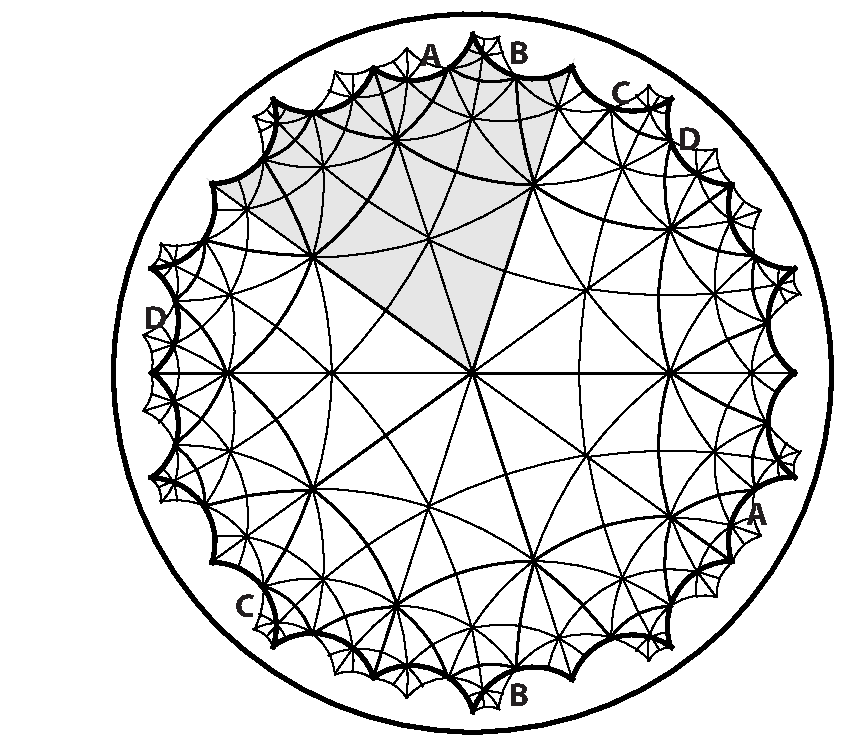
\includegraphics[width=2.75in]{figures/1243_hyp}}}
    \qquad
    \subfloat[Flat 20-gon represents $\omega_1$ of Bring's curve]{{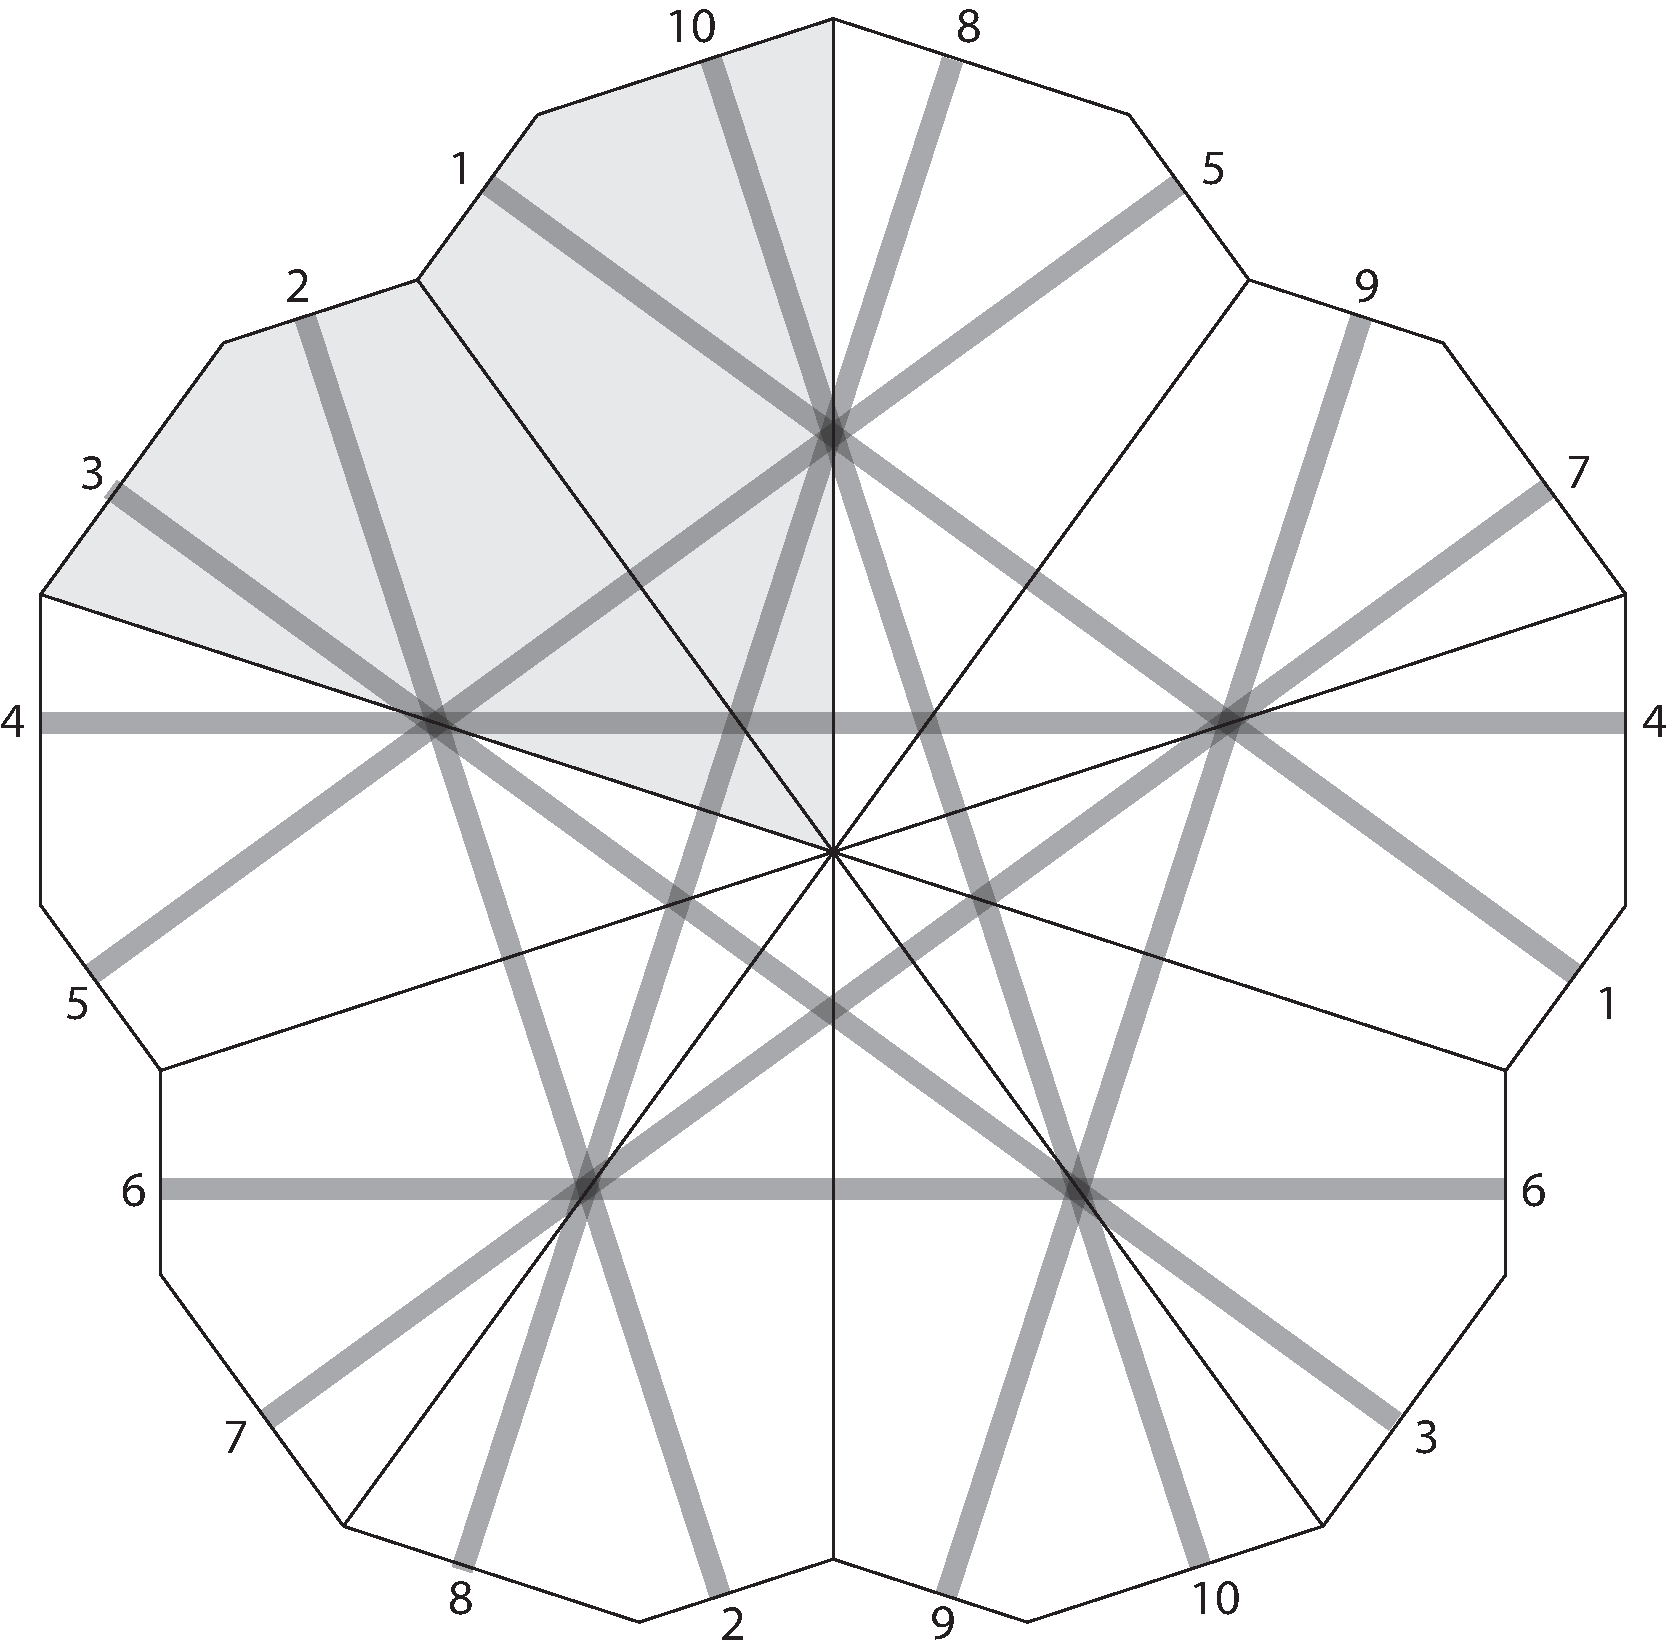
\includegraphics[width=2.75in]{figures/1243_flat}}}%
   \qquad
    \caption{Bring's curve}%
    \label{fig:1331}%
\end{figure}

% need to give credit for both SSD figures


The period matrix of $B$, in its pure form, is calculated in \cite{matti} in Lemma 5.1. %It is well known that $Aut(B) \simeq S_5$, and we reproved it with \texttt{autplane.sage}.


\subsection*{12(1, 4, 7) Schoen's I-WP Surface}

%f6 

In this section, we look at another genus four non-hyperelliptic surface. This surface appears in \cite{dthesis} as an abstract quotient of a triply periodic polyhedral surface where it is called the Octa-8 surface. It is shown in \cite{dthesis} that this curve is a threefold cyclic cover over a six-punctured sphere with branching indices $(1, 1, 1, 1, 1, 1).$ This map is the order-three Gauss map on the minimal surface. The six points are located at the vertices of an octahedron hence the plane curve model is $y^3 - (x^5 - x).$ It is then shown that its conformal structure is compatible to Schoen's I-WP surface.

Its base tessellation is tiled by twenty four $(\frac{\pi}{6}, \frac{\pi}{6}, \frac{\pi}{6})$-triangles. However, after we locate all Weierstrass points, we refine the tessellation as in Figure~\crefformat{figure}{~#2#1{(a)}#3} \cref{fig:147}. The vertices marked as $\bullet$ are Weierstrass points of weight four, those marked as $\circ$ are points of weight one. 


\begin{figure}[htbp]
    \centering
    \subfloat[Hyperbolic Tessellation on I-WP]{{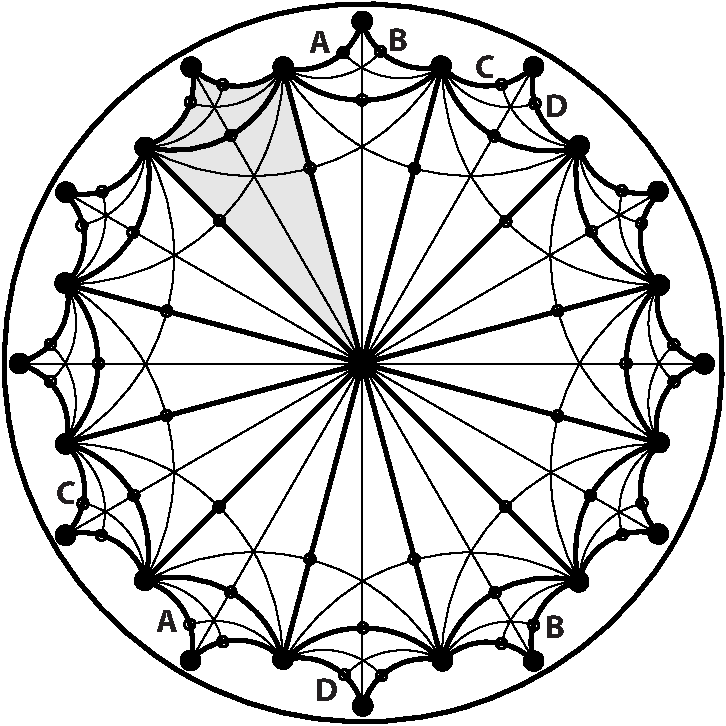
\includegraphics[width=2.75in]{figures/147_weight}}}
    \qquad
    \subfloat[Flat 24-gon represents $\omega_1$ of $12(1, 4, 7)$]{{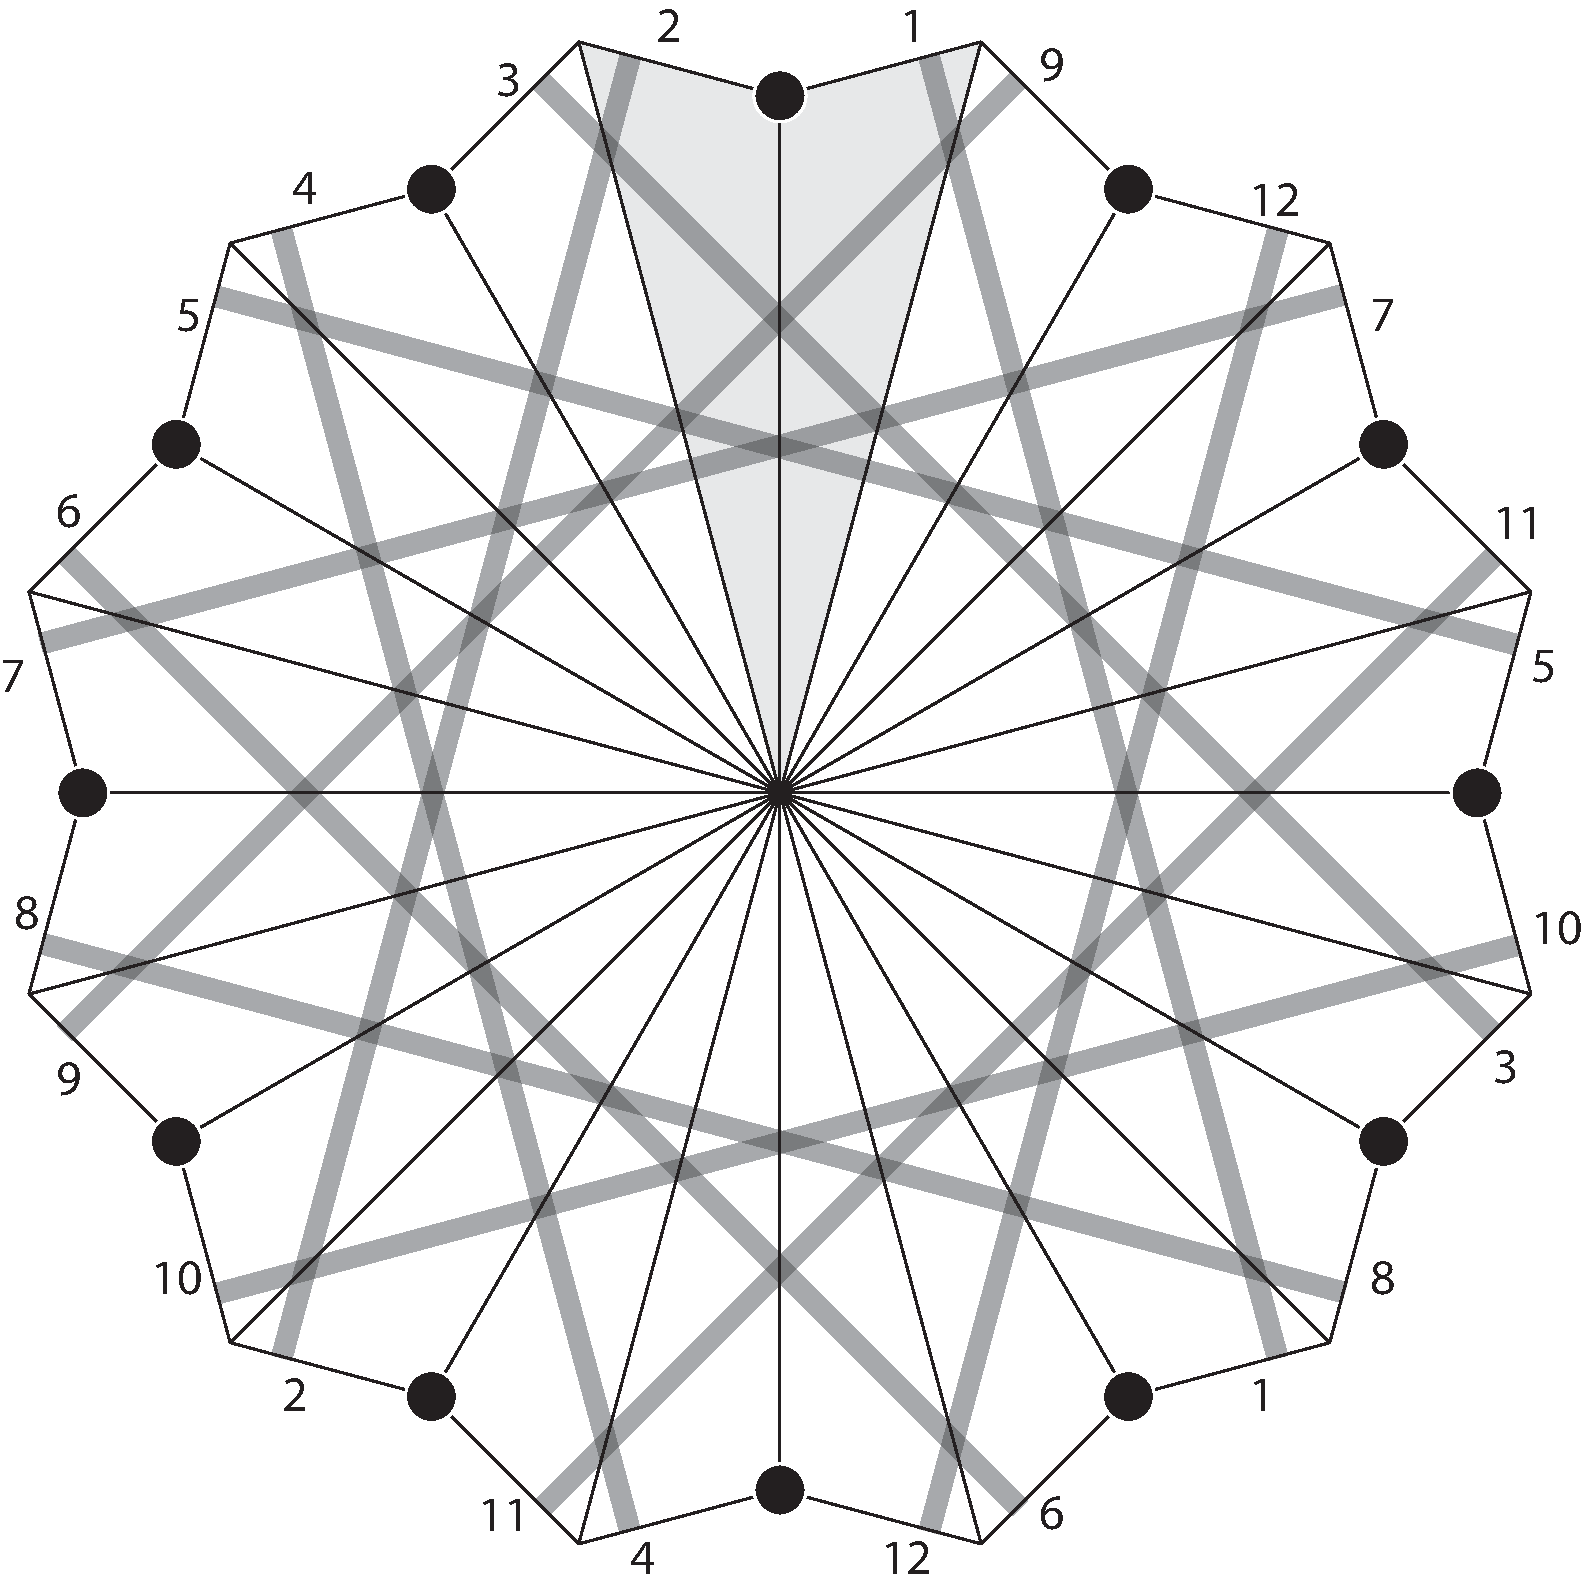
\includegraphics[width=2.75in]{figures/147_flat}}}%
    \qquad
    \caption{Schoen's I-WP surface}
    \label{fig:147}%
\end{figure}


%Considering the orientation of each triangles, we see that we can not choose any two triangles in the tessellation. However, the tessellation can be divided into two congruence classes of 72 triangles each. Given two triangles from the same congruence class, there is one map that maps one triangle to the other. As in $12(1, 3, 8)$ we saw earlier, the weights of the vertices must be preserved. Hence, $|\Aut(\text{I-WP})| = 72.$




%\begin{thm*} $X6$ is nonhyperelliptic and of genus 4. It is shown in the thesis of the first author \cite{dthesis} that this is the Schoen I-WP Surface. \end{thm*} 

%https://ntrs.nasa.gov/archive/nasa/casi.ntrs.nasa.gov/19700020472.pdf


% We present the intersection matrix used to make the period matrix, note it shows that the surface is cyclic.

The period matrix is:

$$\Pi = \begin{pmatrix}
 1 & e^{\frac{\pi i}{6}} & e^{\frac{\pi i}{3}} & i & e^{\frac{2 \pi i}{3}} & e^{\frac{5 \pi i}{6}} & -1 & e^{-\frac{5 \pi i}{6}} \\
 1 & e^{\frac{\pi i}{3}} & e^{\frac{2 \pi i}{3}} & -1 & e^{-\frac{2 \pi i}{3}} & e^{-\frac{\pi i}{3}} & 1 & e^{\frac{\pi i}{3}} \\
 1 & e^{\frac{2 \pi i}{3}} & e^{-\frac{2 \pi i}{3}} & 1 & e^{\frac{2 \pi i}{3}} & e^{-\frac{2 \pi i}{3}} & 1 & e^{\frac{2 \pi i}{3}} \\
 1 & e^{-\frac{5 \pi i}{6}} & e^{\frac{\pi i}{3}} & -i & e^{\frac{2 \pi i}{3}} & e^{-\frac{\pi i}{6}} & -1 & e^{\frac{\pi i}{6}} 
\end{pmatrix}$$
\newpage
 
\subsection*{The modular curve $X_0(63)$}
\label{sec:modular}
Recall that $SL_2(\Z)$ acts transitively on the upper half plane $\mathfrak{h}$ by $\tau \mapsto \frac{a\tau + b}{c\tau + d}$. We quotient the upper half plane by subgroups $\Gamma$ of $SL_2(\Z)$ and metrize the quotient, however, this yields non-compact Riemann surfaces. To get a compact Riemann surface, we consider the extended upper half plane $\mathfrak{h}^{+} := \mathfrak{h} \cup \R \cup \{ \infty \}$ as a subset of $\C P^1$.  

We are most interested in quotients of the upper half plane $\mathfrak{h}^{+}$ by the following subgroups of $SL_2(\Z)$. These subgroups come up naturally in the study of modular forms associated to elliptic curves.

\begin{defn} 
\begin{align*} 
\Gamma_0(N) &:= \left\{ \begin{pmatrix} a & b \\ c & d \end{pmatrix} \in SL_2(\Z) \text{ }  \Big| \text{ } \begin{pmatrix} a & b \\ c & d \end{pmatrix} \equiv  \begin{pmatrix} * & * \\ 0 & * \end{pmatrix} \mod N \right\} \\
\Gamma_1(N) &:= \left\{ \begin{pmatrix} a & b \\ c & d \end{pmatrix} \in SL_2(\Z) \text{ }  \Big| \text{ }  \begin{pmatrix} a & b \\ c & d \end{pmatrix} \equiv  \begin{pmatrix} 1 & * \\ 0 & 1 \end{pmatrix} \mod N \right\} \\
\Gamma(N) &:= \left\{ \begin{pmatrix} a & b \\ c & d \end{pmatrix} \in SL_2(\Z) \text{ }  \Big| \text{ }  \begin{pmatrix} a & b \\ c & d \end{pmatrix} \equiv  \begin{pmatrix} 1 & 0 \\ 0 & 1 \end{pmatrix} \mod N \right\}
\end{align*}
 \end{defn} 

% The automorphism groups of $X(N)$ were found in \cite{bwx} to be $PSL_2(\Z/N\Z)$ (when the genus is greater than 2). The case of all $X_1(N)$ was reportedly found in general in a print, but the second author cannot locate the answer nor a copy of this manuscript. 
The automorphism groups of $X_0(N) := \mathfrak{h}^{+} / \Gamma_0(N)$ were calculated in \cite{km} except for $N=63$. The case of $X_0(63)$ was resolved 2 years later by Noam Elkies \cite{elkies} by two different proofs: a conceptual one that uses enumerative geometry and the modular structure, and an explicit one that exhibits the modular equations. 

%\begin{conjecture} \label{63conj}  All principal polarizations on a Jacobian $J$ coming from curves are found by the method discussed in section ~\ref{sec:find}.  In other words: if there are exactly $n$ curves such that $J \simeq \Jac(C_1) \simeq \Jac(C_n)$, where $C_i \nsimeq C_j$ when $i \neq j$, then the algorithm will find at least the canonical principal polarizations on $J$ associated to $C_1, ..., C_n$.\end{conjecture} 

\begin{conjecture} The program \texttt{CullPB.m} finds all principal polarizations on the curves we consider. \end{conjecture}

If this conjecture is true, it would be a radically different proof than that of Elkies, since we go through computing the automorphism group of the Jacobian of $X_0(63)$. Assuming this conjecture, we go through the proof.

\begin{thm*} $\Aut(X_0(63)) \simeq S_4 \times \Z/2$ \end{thm*} 

\begin{proof} Note the following theorem from \cite{km}: 

\begin{lemma*} $\Aut(X_0(63))$ is either $A_4 \times \Z/2$ or $S_4 \times \Z/2$. 
\end{lemma*}

Using the period matrix provided by Mascot, performed with 150 precisions, \texttt{autperio.sage} gives (using Conjecture ~\ref{63conj}):

\begin{lemma*} $\Aut(X_0(63))$ is either $C_2^{\text{ }4}$ or $S_4 \times \Z/2$.
\end{lemma*}

Therefore, it must be that $\Aut(X_0(63)) \simeq S_4 \times \Z/2$. 
\end{proof} 
%add citation for this paper etc. 

\vspace{+10pt} 
The period matrix used in our calculation of $\Aut(\Jac(X_0(63)), p_i)$ was computed by Nicolas Mascot using an alteration of his personal code.

\begin{remark} Mascot's paper \cite{n} discusses finding the period matrices for $X_1(N)$ by integrating cuspforms along modular symbols. His algorithm works for any compactified modular curve, but it works best when $N$ is square-free. In the non-squarefree case, the coefficients in the $q$-expansions of the cuspforms and the $j$-invariant do not converge as quickly, thus they require more digits of precision. \end{remark}

\begin{remark} In private correspondence, John Voight programmatically proved that $X_0(63)$ is not a cyclically branched cover of the sphere. He showed that the list of dimensions of the space of $H$-invariant differentials on $X_0(63)$ where $H$ is a cyclic subgroup of $Aut(X_0(63))$, does not contain zero. Note that the genus of the quotient $X_0(63)/H$ is equal to the dimension of the $H$-invariant differentials.
 \end{remark} 


\begin{comment}
Note that this calculation is peformed with 150 prec. For ease on the eye, we list here only 8 digits of accuracy. 
\begin{align*} 
a &= 2.8369265\\
b &= 0.79658094\\c 
&= 1.0418064\\
d &= 2.0836128\\
e &= 1.8044616\\
f &= 1.1033105\\
g &= 1.5931619\\
h &= 1.2739932\\
k &= 1.9109898\\
\ell &= 0.60148720 \\
m &= 0.38007609\\
n &= 2.9728805 \\ 
o &= 0.79658094 \\ 
p &= 3.2170027 \\ 
q &= 1.7985394 \\ 
r &= 2.4568505 \\ 
s &= 1.3797187 \\
t &= 4.5660424 \\
u &= 3.7694615 \\
v &= 1.0383872 \\
w &= 2.1762996
\end{align*} 


$$(\Pi) := \begin{pmatrix}
-m + bi & 
-a & 
a & 
\frac12a + mi & 
a + gi & 
p + bi & 
\frac12 a - si & 
gi & 
-a & 
-q - wi\\
-f - ci 
& -di 
& -di 
& f - ci
&  0 
& -f - ci
& f - ci & -di
& di
& -2f \\
-m - \frac12 ai& -g & g& o - mi& g - ai& t - \frac12 ai& o - ri& -ai& -g& -u - vi 
\\
-ki& 0& -e - ki& -e - ki& -e & -e& -e& -ki& -ki& -ki
\\
-\ell  - hi& -hi& \ell  - \frac12 hi& 0& \ell & \frac12 hi& -\frac12 hi& -\frac12 hi& -\frac12 hi& -\frac12 hi
\end{pmatrix}$$

\end{comment}

\section{Closing Remarks}
\label{sec:questions}

We speak here of polarizations up to auto-equivalence and ask natural questions on Jacobians with multiple principle polarizations, answering all but one of the questions using methods developed in our paper.

We fix some notation. Let $\theta_C$ be the canonical principal polarization of $\Jac(C)$ with respect to $C$. We call $\Aut(A, a_i)$ a symplectic automorphism group of $A$, as the automorphisms respect the principal polarization $a_i$, which is a symplectic form on $A$.

\begin{question} $\Aut(\Jac(C), \theta_C)$ will have the highest order of all symplectic automorphism groups of $\Jac(C)$. \end{question}

This is proven false by example $12(1,5,6)$, where $|\Aut(\Jac(12(1, 5, 6)), \phi_{12(1, 5, 6)})| = 24$, but $|\Aut(\Jac(12(1, 5, 6)), a_i)| = 32$ is achieved. It is more dramatically proven false by Schoen's I-WP Surface, where $|\Aut(\Jac(\text{I-WP}), \phi_{\text{I-WP}})| = 288$, but $|\Aut(\Jac(\text{I-WP}), a_i)|$ achieves $576$ and $864$.

\begin{question} Principal polarizations $p_1$ and $p_2$ are auto-equivalent if and only if they are analytically equivalent. In other words, $$\Aut(X, p_1) \simeq \Aut(X, p_2) \Leftrightarrow p_1 = p_2$$ \end{question}

The direction ($\Leftarrow$) is clear because $\mc{L}$ and $\mc{M}$ are analytically equivalent if and only if $c_1(\mc{L}) = c_1(\mc{M})$ by [BL 2.5.3]. The other direction is false.  This is proven false by the following two \textit{non-isomorphic} curves with the same (unpolarized) Jacobian from Theorem 1  \cite{howe1}:

$$X: 3y^2 = (2x^2- 2)(16x^4 + 28x^2 + 1)$$ 

$$X': -y^2 = (2x^2 + 2)(16x^4 + 12x^2 + 1)$$ 

which both have $\Aut(\Jac(X), \theta_X)\simeq C_2 \times C_2 \simeq \Aut(\Jac(X'), \theta_{X'})$. %This is true for many curves in Howe's first family where $t \in \Z^\times$. 

%First, note that $$\Aut(\Jac(X), c_1(\mc{L})) \simeq \Aut(\Jac(X), c_1(\mc{M}))$$ does not immediately imply that $c_1(\mc{L}) = c_1(\mc{M})$.

\begin{question} If $\Jac(C) \simeq \Jac(C')$ as complex varieties, then $$\Aut(\Jac(C), \theta_C) \simeq \Aut(\Jac(C'), \theta_{C'})$$  \end{question} 

We checked this question on the family of hyperelliptic cases of genus 2 from \cite{howe1} Theorem 1, where it is true. However, there is no reason to expect this to be true in general. Yet, we cannot disprove it easily. 
% tktk 
% change this to conjecture if we are not providing an answer



\begin{thebibliography}{9}

\bibitem{jeroen}
N. Bruin, J. Sijsling, A. Zotine,
\textit{Numerical Computation of Endomorphism Rings of Jacobians},
\texttt{https://arxiv.org/pdf/1807.02605.pdf}, preprint.

\bibitem{Torelli}
K. Lauter, J.-P., Serre, 
\textit{Geometric Methods for Improving the Upper Bounds on the Number of Rational Points on Algebraic Curves over Finite Fields}, 
Journal of Algebraic Geometry,
Vol. 10, 2001.


\bibitem{finn}
H. Martens
\textit{A New Proof of Torelli's Theorem},
Annals of Mathematics,
Second Series, Vol. 78, No. 1, 1963, pp.107--111.

\bibitem{oe}
A. Weil,
\textit{Oeuvres Scientifiques},
Springer,
Vol. 2. 


\bibitem{bl} 
C. Birkenhake, H. Lange, 
\textit{Complex Abelian Varieties},
Springer, 2004.


\bibitem{dami} 
D. Lee,
\textit{On a triply periodic polyhedral surface whose vertices are Weierstrass points}
Arnold Mathematical Journal, 
Vol. 3, Issue 3, 2017, pp.319--331.

\bibitem{dthesis} 
D. Lee, 
\textit{Geometric realizations of cyclically branched coverings over punctured spheres}
\texttt{https://arxiv.org/abs/1809.06321}, preprint.


\bibitem{matti} 
M. Weber,
\textit{Kepler's small stellated dodecahedron as a Riemann surface}
Pacific Journal of Mathematics, 
Vol. 220, 2005, pp.167--182.



%did we use these other guys?

%https://arxiv.org/pdf/math/0508458.pdf might be useful



\bibitem{nn} 
M. S. Narasimhan, M. V. Nori,
\textit{Polarisations on an abelian variety},
Proceedings of the Indian Academy of Sciences,
Vol. 90, 1951, pp.125--128.




\bibitem{[GAP2018]}
\textit{Small Groups Package}
\texttt{The GAP Group, GAP -- Groups, Algorithms, and Programming, Version 4.9.1; 2018.}
\textit{https://www.gap-system.org}



\bibitem{kw}
H. Karcher, M. Weber,
\textit{On Klein's Riemann Surface}
The Eightfold Way, MSRI Publications, 
Vol. 35, 1998, pp.9--49.


\bibitem{hyp}
R. Lercier, C. Ritzenthaler, and J. Sijsling,
\textit{Fast computation of isomorphisms of hyperelliptic curves and explicit Galois descent}
Proceedings of the Tenth Algorithmic Number Theory Symposium, 2013, pp. 463–-486.

\bibitem{several} 
H. Lange,
\textit{Abelian Varieties with Several Principal Polarizations},
Duke Mathematical Journal,
Vol. 55, Number 3, 1987, pp.617--628.

\bibitem{howe1}
E. Howe,
\textit{Constructing Distinct Curves with Isomorphic Jacobians},
Journal of Number Theory,
Vol. 56, Issue 2, 1996, pp.381--390.

\bibitem{howe2} 
E. Howe,
\textit{Infinite families of pairs of curves over $\Q$ with Isomorphic Jacobians},
Journal of the London Mathematical Society,
Vol. 72, Issue 2, 2005, pp.327--350.

\bibitem{iko}
T. Ibukiyama, T. Katsura, and F. Oort,
\textit{Supersingular curves of genus two and class numbers},
Composito Mathematica,
Vol. 57, No. 2, 1986, pp.127--152.

\bibitem{km}
M. A. Kenku and F. Momose,
\textit{Automorphism Groups of the modular curves $X_0(N)$},
Composito Mathematica,
Vol. 65, No. 1, 1988, pp.51--80.
 
\bibitem{elkies}
N. Elkies,
\textit{The automorphism group of the modular curve $X_0(63)$},
Composito Mathematica,
Vol. 74, 1986, pp.127--152.

\bibitem{n}
N. Mascot,
\textit{Computing modular Galois representations}
Rendiconti del Circolo Matematico di Palermo,
Vol. 62, Issue. 3, 2013, pp.451--476.

\bibitem{bwx}
F. Bars, A. Kontogeorgis, and X. Xarles,
\textit{Bielliptic and Hyperelliptic Modular Curves $X(N)$ and the group $Aut(X(N))$},
Acta Arithmetica,
Vol. 161, Issue 3, 2012.

\begin{comment}
\bibitem{mestre}
J-F. Mestre
\textit{Corps euclidiens, unit\'es exceptionnelles et courbes \'elliptiques. }
J.Number Theory 13 (1981), 123-137
\end{comment} 
\end{thebibliography}





%Cite: F. Momose, Automorphism groups of the modular curves X1(N).}

\end{document}
\grid
\grid
\grid
